\documentclass{article}
\usepackage[backend=biber]{biblatex}
\usepackage{graphicx}
\usepackage[colorlinks=true]{hyperref}
\usepackage{booktabs}
\usepackage{siunitx}
\usepackage[]{amsmath}
\usepackage{gensymb}
\usepackage{mathtools}
\usepackage{fancyref}
\addbibresource{/home/giorgio/Bibliography/bibliography.bib}
\hypersetup{
    colorlinks=true,
    linkcolor=blue,
    filecolor=magenta,  
    citecolor=blue,    
    urlcolor=cyan,
    pdftitle={Turbina ad alta temperatura},
    bookmarks=true,
}

\author{Giorgio De Trane, \\Anthony S. Luna Gonzales, \\Giulia Barbero, \\Roberto Giusto}
\title{\textbf{Turbina ad alta temperatura}}

\begin{document}
    \setlength{\parindent}{0pt}
    \maketitle
    \begin{center}
        
\includegraphics[width=0.8\textwidth]{Sources/polito_logo.png}\linebreak\newline
       \textbf{\textit{Materiali per applicazioni aerospaziali}}\linebreak\newline
        \textit{Gruppo di lavoro n. 10B}\linebreak\newline
        \textit{Anno accademico 2020/2021}
    \end{center}

    \newpage
    \tableofcontents
    \newpage
    \section{Introduzione\label{Intro}}
    I turbomotori assiali aeronautici possono essere suddivisi, generalmente, in tre macrosezioni
    fondamentali: compressore, camera di combustione e turbina.\\

    \begin{figure}[h!]
        \centering
        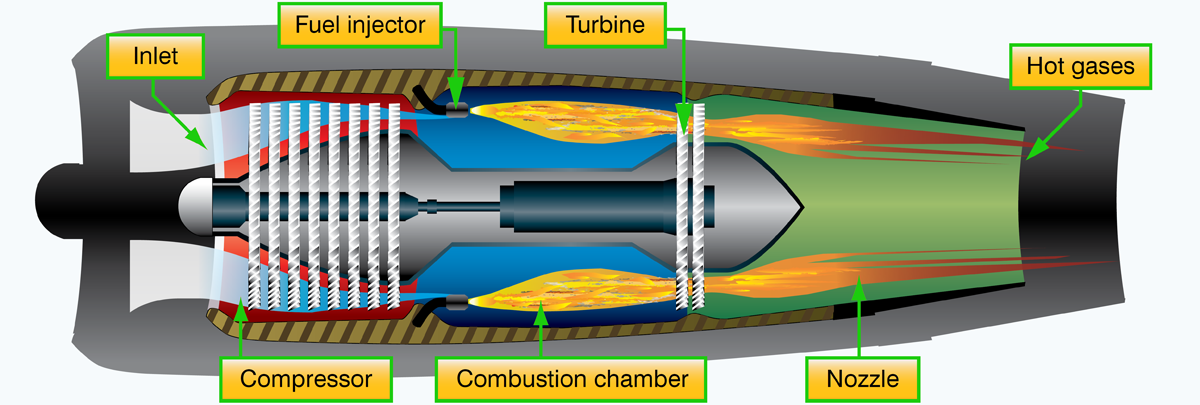
\includegraphics[width=0.8\textwidth]{Sources/turbojet.png}\\
    \caption{Schema generale di un motore turbojet \autocite*{turbojet}} 
    \end{figure}

    Un \textit{inlet} favorisce l'afflusso di aria esterna al \textit{compressore}, il quale
    la comprime in un volume nettamente inferiore, attraverso vari stadi alternati di pale rotoriche-statoriche.\\
    L'aria fortemente compressa viene poi miscelata con il carburante iniettato in \textit{camera di combustione},
    in una determinata proporzione (dipendente da vari fattori): la miscela viene quindi combusta, seguendo le trasformazioni di
    un preciso ciclo termodinamico (ogni motore ha la sua implementazione, ma i principi fondamentali sono gli stessi), causando un repentino
    aumento di pressione e temperatura.\\
    Successivamente, i gas combusti vengono espansi rapidamente dalla \textit{turbina} (la quale, inoltre, mette in rotazione l'albero di trasmissione), attraverso, in questo caso,
    vari stadi alternati di pale statoriche-rotoriche.\\
    Infine, i gas espansi vengono espulsi e accelerati attraverso un \textit{ugello}.\\
    Tutto il processo fornisce una spinta, secondo il principio di azione-reazione \autocite*{Aircr_engine_design}.\\ \\
    Le temperature e le sollecitazioni raggiunte dalle palette di turbina sono tipicamente in range estremi (in particolare per gli stadi ad alta pressione),
    al punto che la scelta dei materiali é sostanzialmente diversa da quella del compressore.\\
    In un moderno jet engine, si possono raggiungere temperature massime che eccedono i 1500 °C \autocite*{SciencePubGroup}, 
    senza contare le sollecitazioni meccaniche a cui sono sottoposte le pale HP, a causa di pressioni elevatissime,
    forze centrifughe per velocitá di migliaia di RPM e intense vibrazioni, nonché problemi di corrosione
    e reazioni chimiche indesiderate, favorite oltretutto dall'alta temperatura.\\

    \begin{figure}[h!]
        \centering
        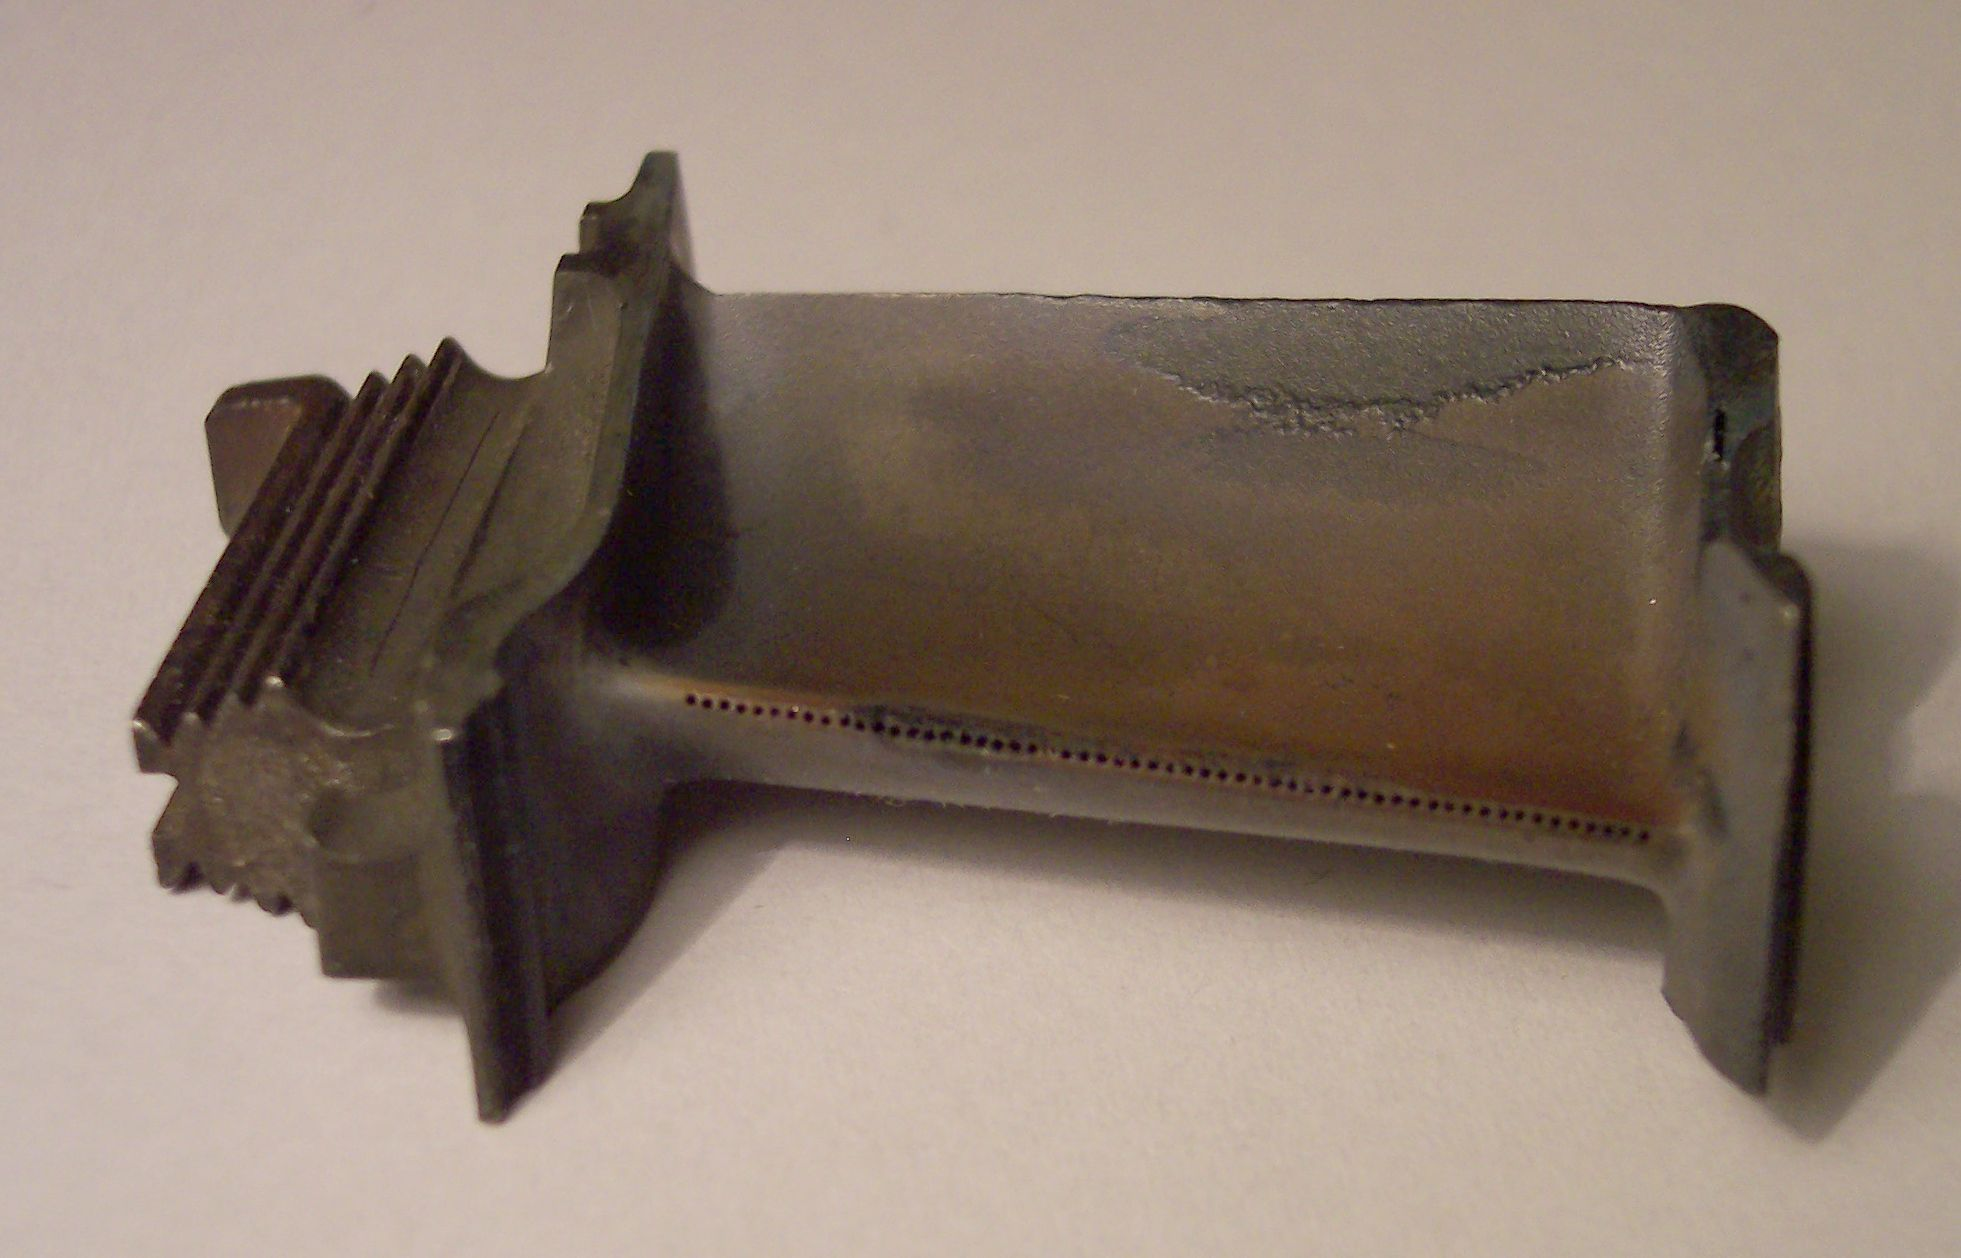
\includegraphics[width=\textwidth]{Sources/Turbinenschaufel_RB199.jpg}
        \caption{Effetti dell'ambiente operativo estremo su una paletta di turbina \autocite*{turbine_blade}}
        \phantomsection \label{fig:paletta_logorata}
    \end{figure}

    É necessario, dunque, scegliere un materiale (o una combinazione di piú materiali)
    in grado di sopportare, per il tempo di operativitá del componente, l'effetto
    simultaneo dell'elevatissima temperatura, dell'aggressivitá chimica e delle sollecitazioni meccaniche istantanee e cicliche,
    tenendo in considerazione, eventualmente, la possibilitá di un raffreddamento attivo.\\

    \clearpage






    \section{Funzioni, obiettivi, vincoli\label{Funzioni_ob_vinc}}

    Utilizzando lo sconfinato database interattivo fornito dal software \textit{Granta EduPack}
    ed includendovi inizialmente tutti i materiali del terzo livello, sono stati imposti dei vincoli 
    tali da soddisfare diversi obiettivi molto stringenti, sorti dalla necessitá di costruire un componente
    in grado di operare in un ambiente cosí ostile, come descritto nelle sezioni \ref{Intro} e \ref{superleghe_mot_aer} e riassunto nella
    tabella (\ref{tab:funz_ob_vinc}).
    
        \begin{table}[h!]
        \centering
        \begin{tabular}{@{}c|c@{}}
        \toprule
        \textbf{Funzioni} &
          Produzione di palette per stadi di turbina HP \\ \midrule
        \textbf{Obiettivi} &
          \begin{tabular}[c]{@{}c@{}}Ottima resistenza a frattura\\ Ottima resistenza a fatica\end{tabular} \\ \midrule
        \textbf{Vincoli} &
          \begin{tabular}[c]{@{}c@{}}$ T_{max} \ \approx 1100 \  _{}^{\circ}\textrm{C}$ \\ $ K_{1c} > 30 \ MPa \cdot m^{0.5}$ \\ $ \sigma_e > 360 \  MPa$ \\ Resistenza all'ossidazione: ottima\\ Processo produttivo: investment casting\\ Percentuale di materiale riciclabile: fino al 30\%\end{tabular} \\ \bottomrule
        \end{tabular}
        \caption{Funzioni, obiettivi e vincoli di progetto}
        \label{tab:funz_ob_vinc}
        \end{table}
    
    Come giá detto nelle sezione \ref{Intro}, l'ambiente estremamente ostile necessita l'imposizione di vincoli molto 
    rigidi, a partire dalla temperatura di esercizio e dalla resistenza all'ossidazione, fino a vincoli di natura
    meccanica.

    In particolare, ci si é focalizzati sulla \textit{fracture toughness} e sulla \textit{resist fatigue} che, 
    come verrá approfondito in sezione \ref{material_index}, sono poi le due grandezze scelte per valutare le performance
    tramite indici di merito.

    La \textit{fracture toughness} é un parametro estremamente importante, in quanto consente di valutare in maniera quantitativa
    la resistenza alla propagazione di una cricca. 
    
    Nel caso in cui una cricca dovesse verificarsi e superare una certa dimensione critica, una corretta valutazione
    di questo requisito ne impedisce la propagazione repentina, col rischio di failure incontenibile.

    A questa grandezza é inevitabilmente legata la \textit{resist fatigue}. Tali cricche sono infatti generate da carichi ciclici,
    spesso di magnitudine decisamente inferiore alla \textit{ultimate tensile strength} del materiale, per cui un'elevata
    resistenza a fatica é di vitale importanza per componenti soggetti a vibrazioni e sollecitazioni cicliche prolungate.

    Dato che giá preliminarmente il database ha scartato materiali non appartenenti alla famiglia delle leghe, é stato imposto
    un ulteriore vincolo sul processo produttivo. Si é optato per l'\textit{investment casting} piuttosto che per 
    l'\textit{additive manufacturing} (approfondimento in sezione \ref{Casting}), per favorire un rateo di produzione molto elevato, che possa col tempo ammortizzare
    gli enormi investimenti iniziali che questa scelta comporta.

    Seppur non al livello dell'AM, questo processo produttivo porta a un ridotto spreco di materiale
    rispetto ad altre tecniche sottrattive. 

    Oltre a rappresentare un potenziale risparmio economico, la riduzione di materiale sprecato é un obiettivo
    chiave (tra i tanti) per la sostenibilitá ambientale, verso cui anche le aziende aerospaziali stanno 
    adottando e intensamente pianificando un approccio piú sostenibile per il futuro, in virtú di motivazioni etiche
    e anche delle normative in merito, con gli anni sempre piú severe ed esigenti.

    Alla luce di queste considerazioni e di quanto visto in risorse come l'\textit{European Aviation Environmental Report} (2019)
    di \textit{EASA} \autocite{EASA_environ_report_2019} o in \textit{Best Industry Practices for Aircraft Decommissioning (BIPAD)}
    dell'\textit{IATA} \autocite{IATA_aircraft_decomm}, si é deciso di imporre come requisito di progetto 
    una percentuale di riciclabilitá del 30\%, per il materiale target.

    \begin{figure}[h!]
        \centering
        \phantomsection
        \label{fig:fatigue_vs_density}
        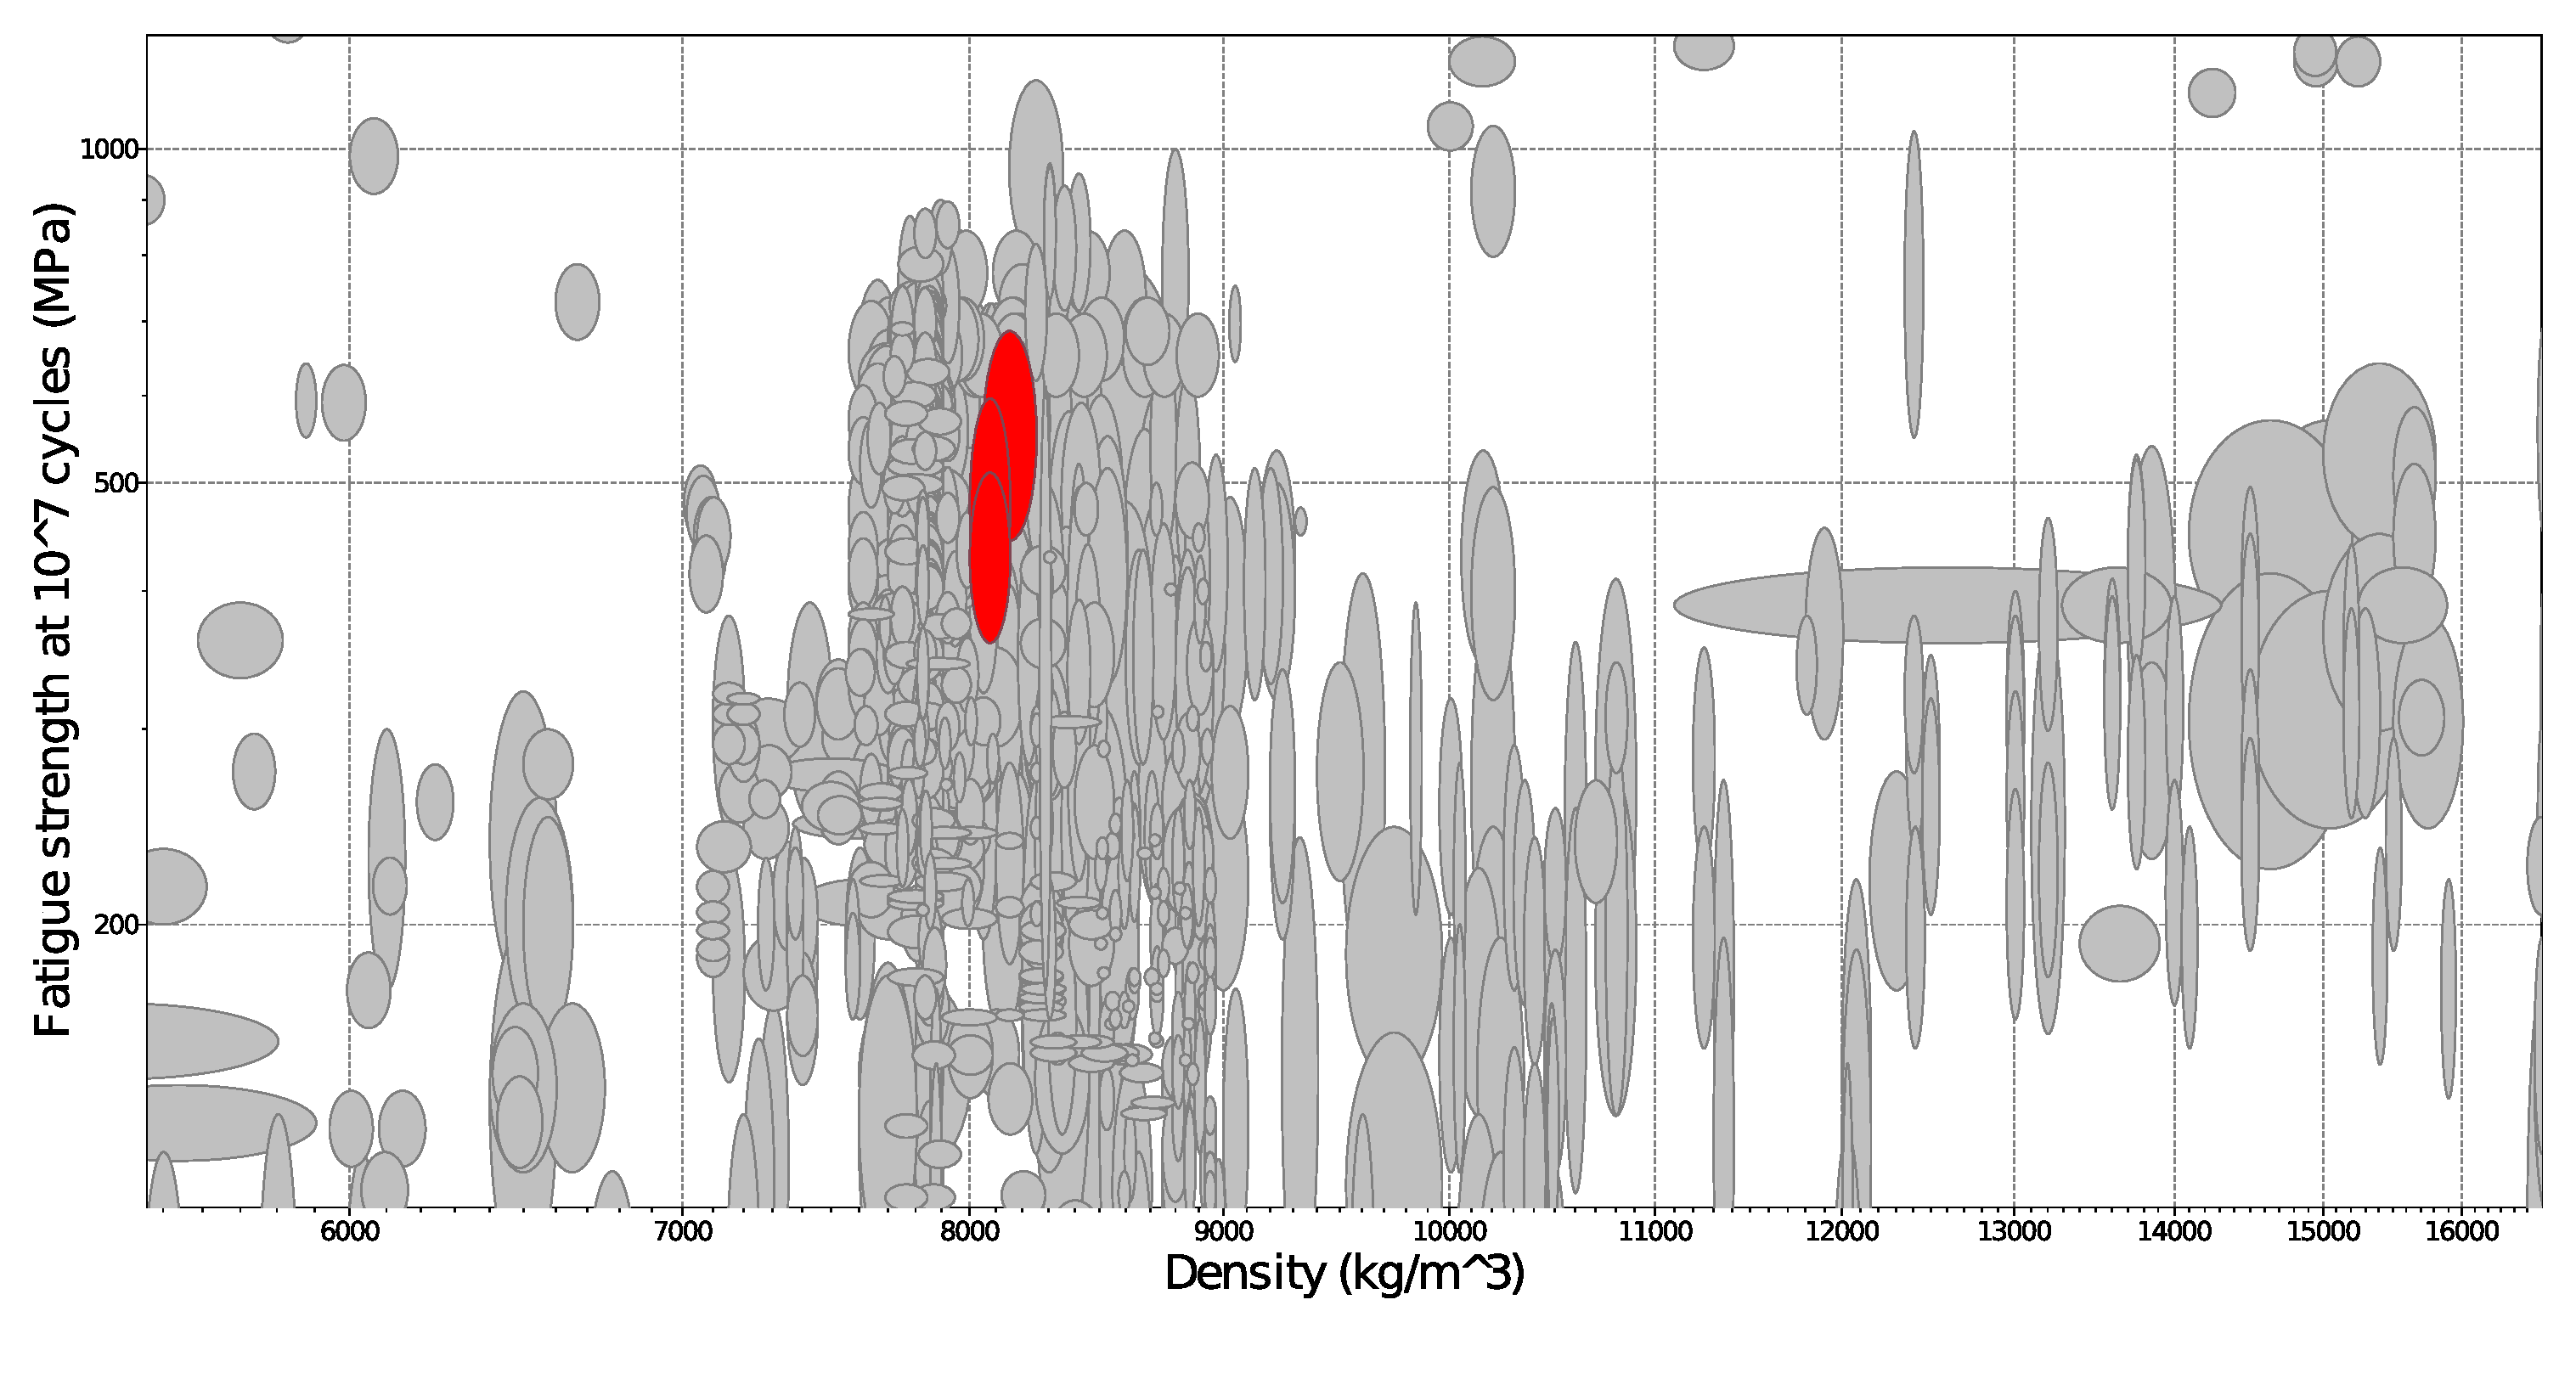
\includegraphics[width=0.70\textwidth]{fatigue.eps} 
        \caption{Fatigue vs Density}       
    \end{figure}

    \begin{figure}[h!]
        \centering
        \phantomsection
        \label{fig:fatigue_vs_density}
        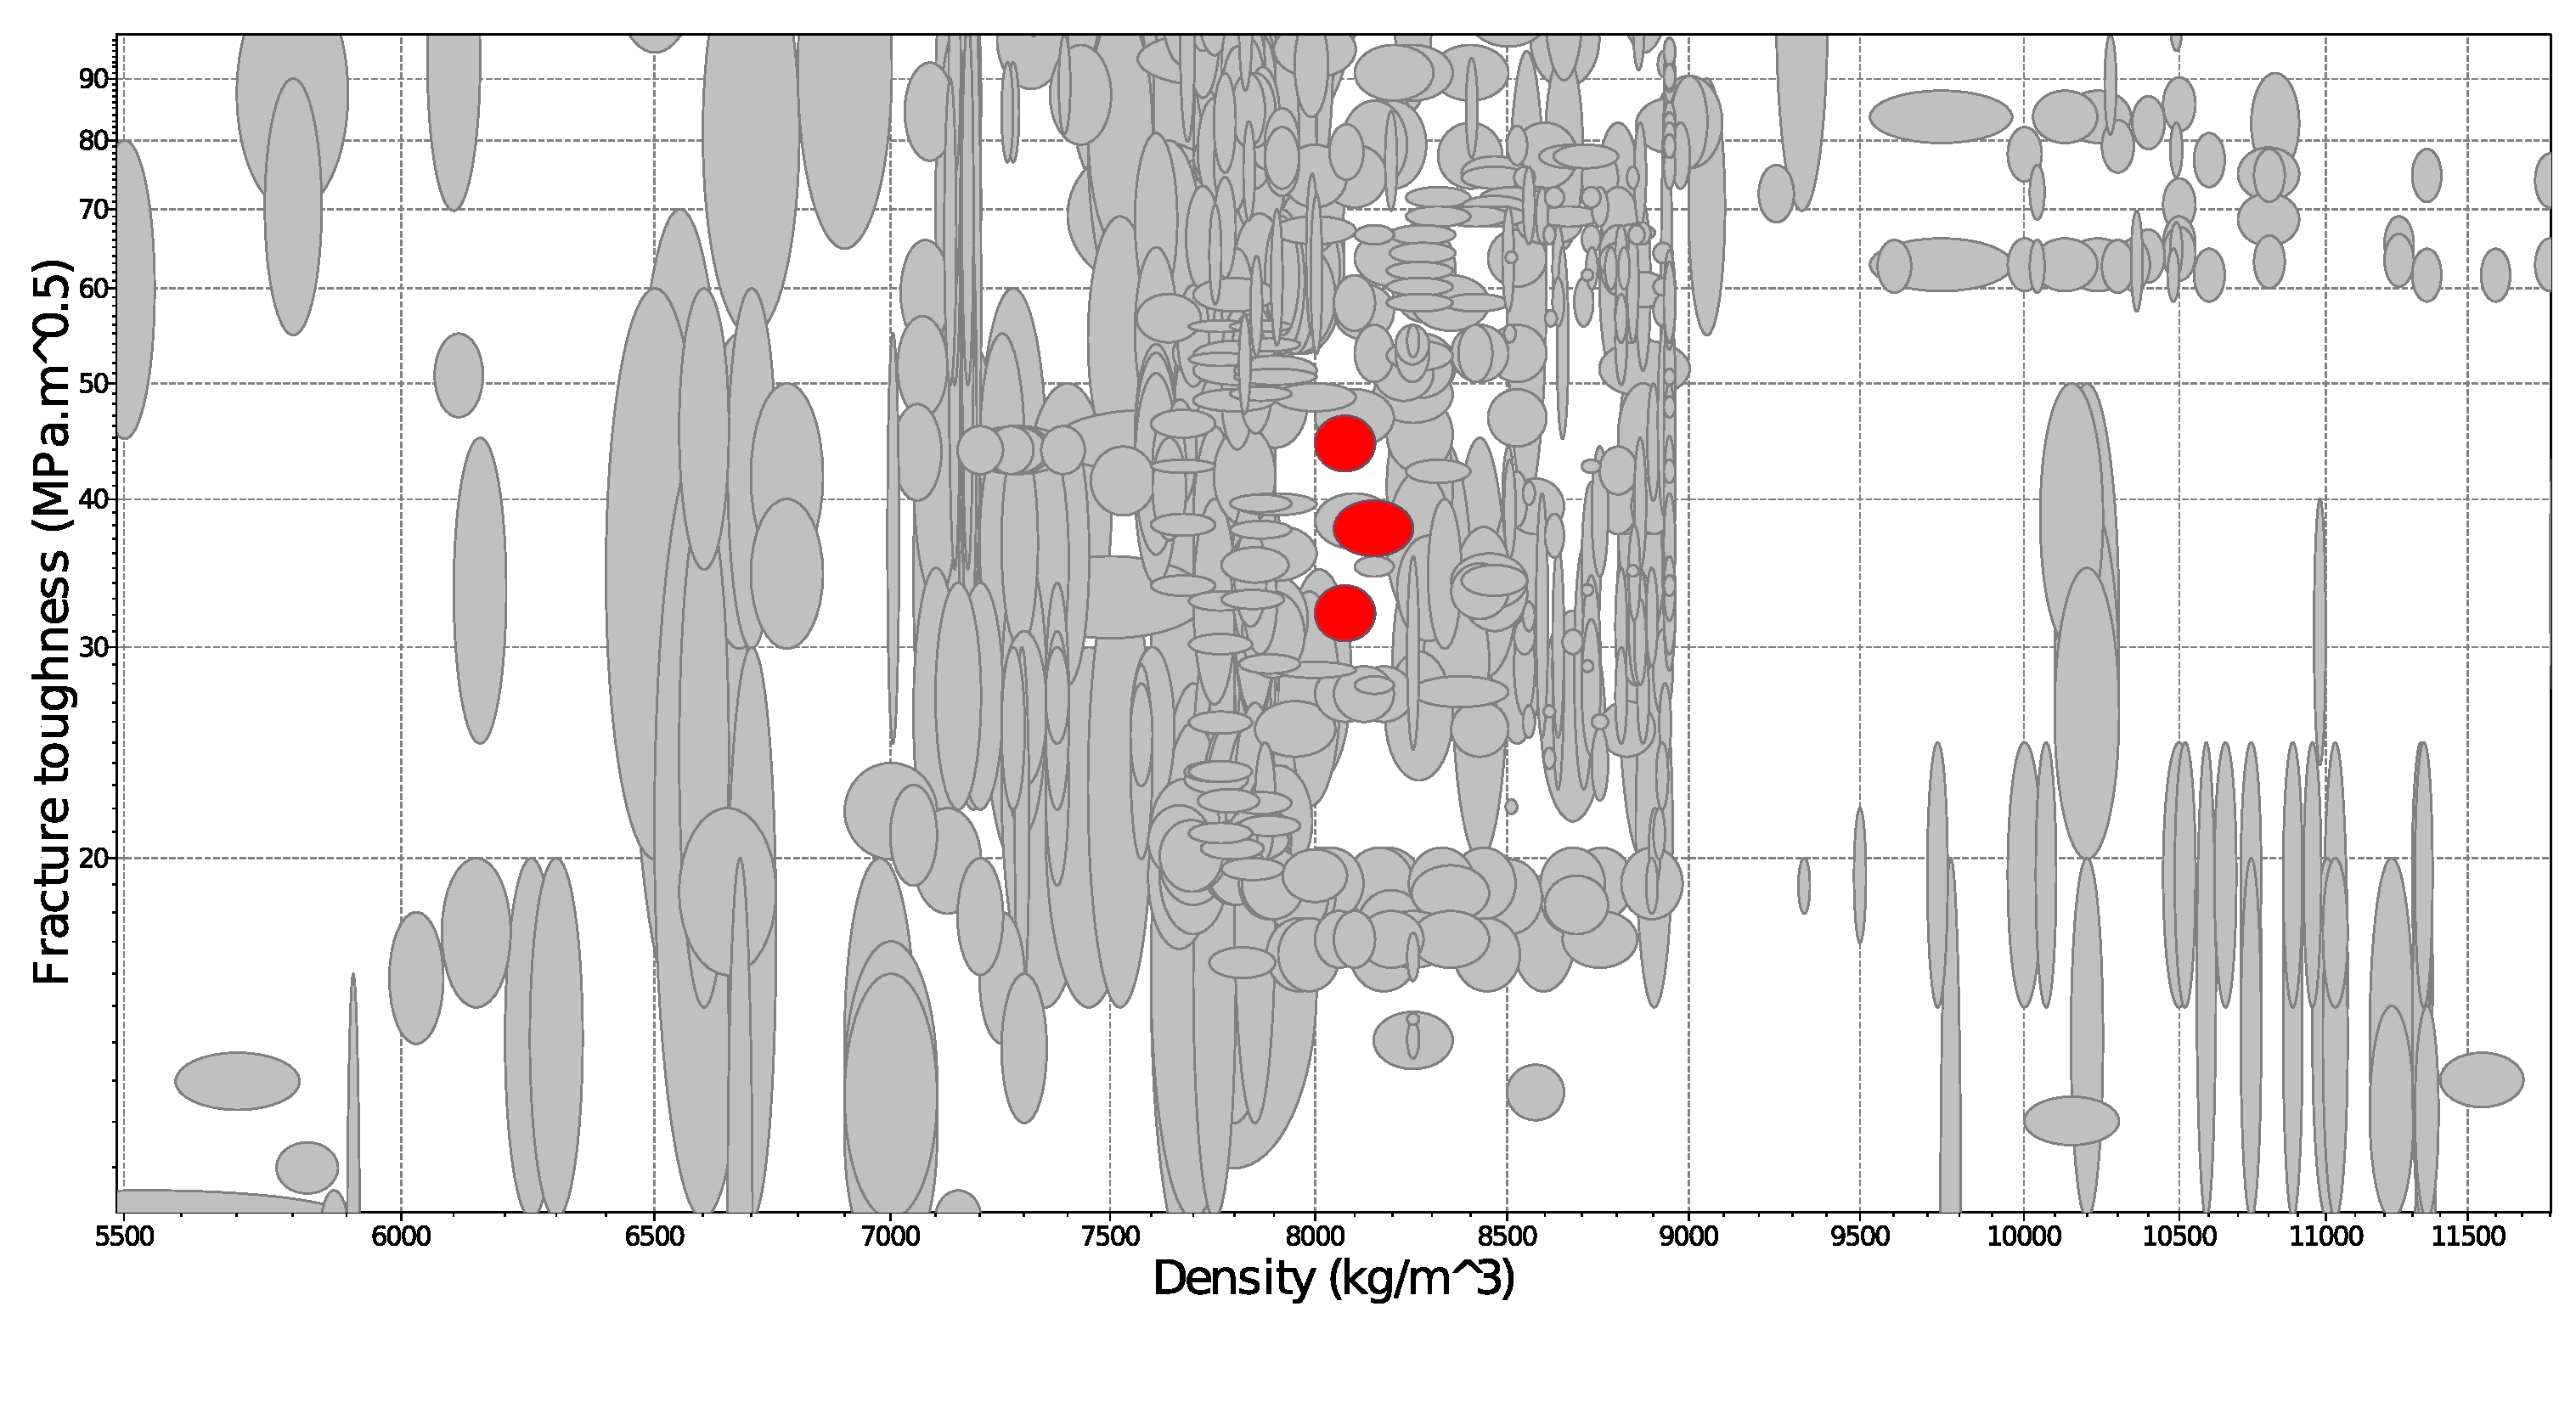
\includegraphics[width=0.68\textwidth]{fracture_toughness.eps} 
        \caption{Fracture Toughness vs Density}       
    \end{figure}

    Come si puó notare, i vincoli imposti hanno messo in evidenza tre potenziali materiali candidati, appartenenti
    alla famiglia delle superleghe di nickel (approfondimento in sezione \ref{superleghe_mot_aer}).



    \clearpage 

    \section{Superleghe nei motori aeronautici\label{superleghe_mot_aer}}
  
    L'evoluzione esponenziale del settore aerospaziale e di tutte le discipline satelliti, 
    nel corso degli ultimi decenni, vede sicuramente la scienza dei materiali 
    tra i suoi driving factors.

    Tra le infinite innovazioni, un ruolo essenziale é sicuramente giocato dalle \textit{superleghe}.

    Tali leghe metalliche sono cosí definite poiché possono tipicamente raggiungere
    una temperatura di esercizio pari a circa il 70-80 \% della propria temperatura di 
    fusione, anche per periodi piuttosto prolungati, pur mantenendo eccezionali
    proprietá meccaniche.
    \\ 

    In commercio sono disponibili una moltitudine di superleghe, tra cui quelle basate 
    sul Nickel, sul Titanio, sul Cobalto e molte altre.
    Viste le elevatissime temperature di esercizio delle palette di turbina HP, le
    uniche superleghe con cui al momento sono prodotte, sono proprio quelle a base di Nickel
    e, piú recentemente, anche Cobalto. 
    
    \begin{figure}[h!]
        \centering
        \phantomsection \label{turbofan_drawing}
        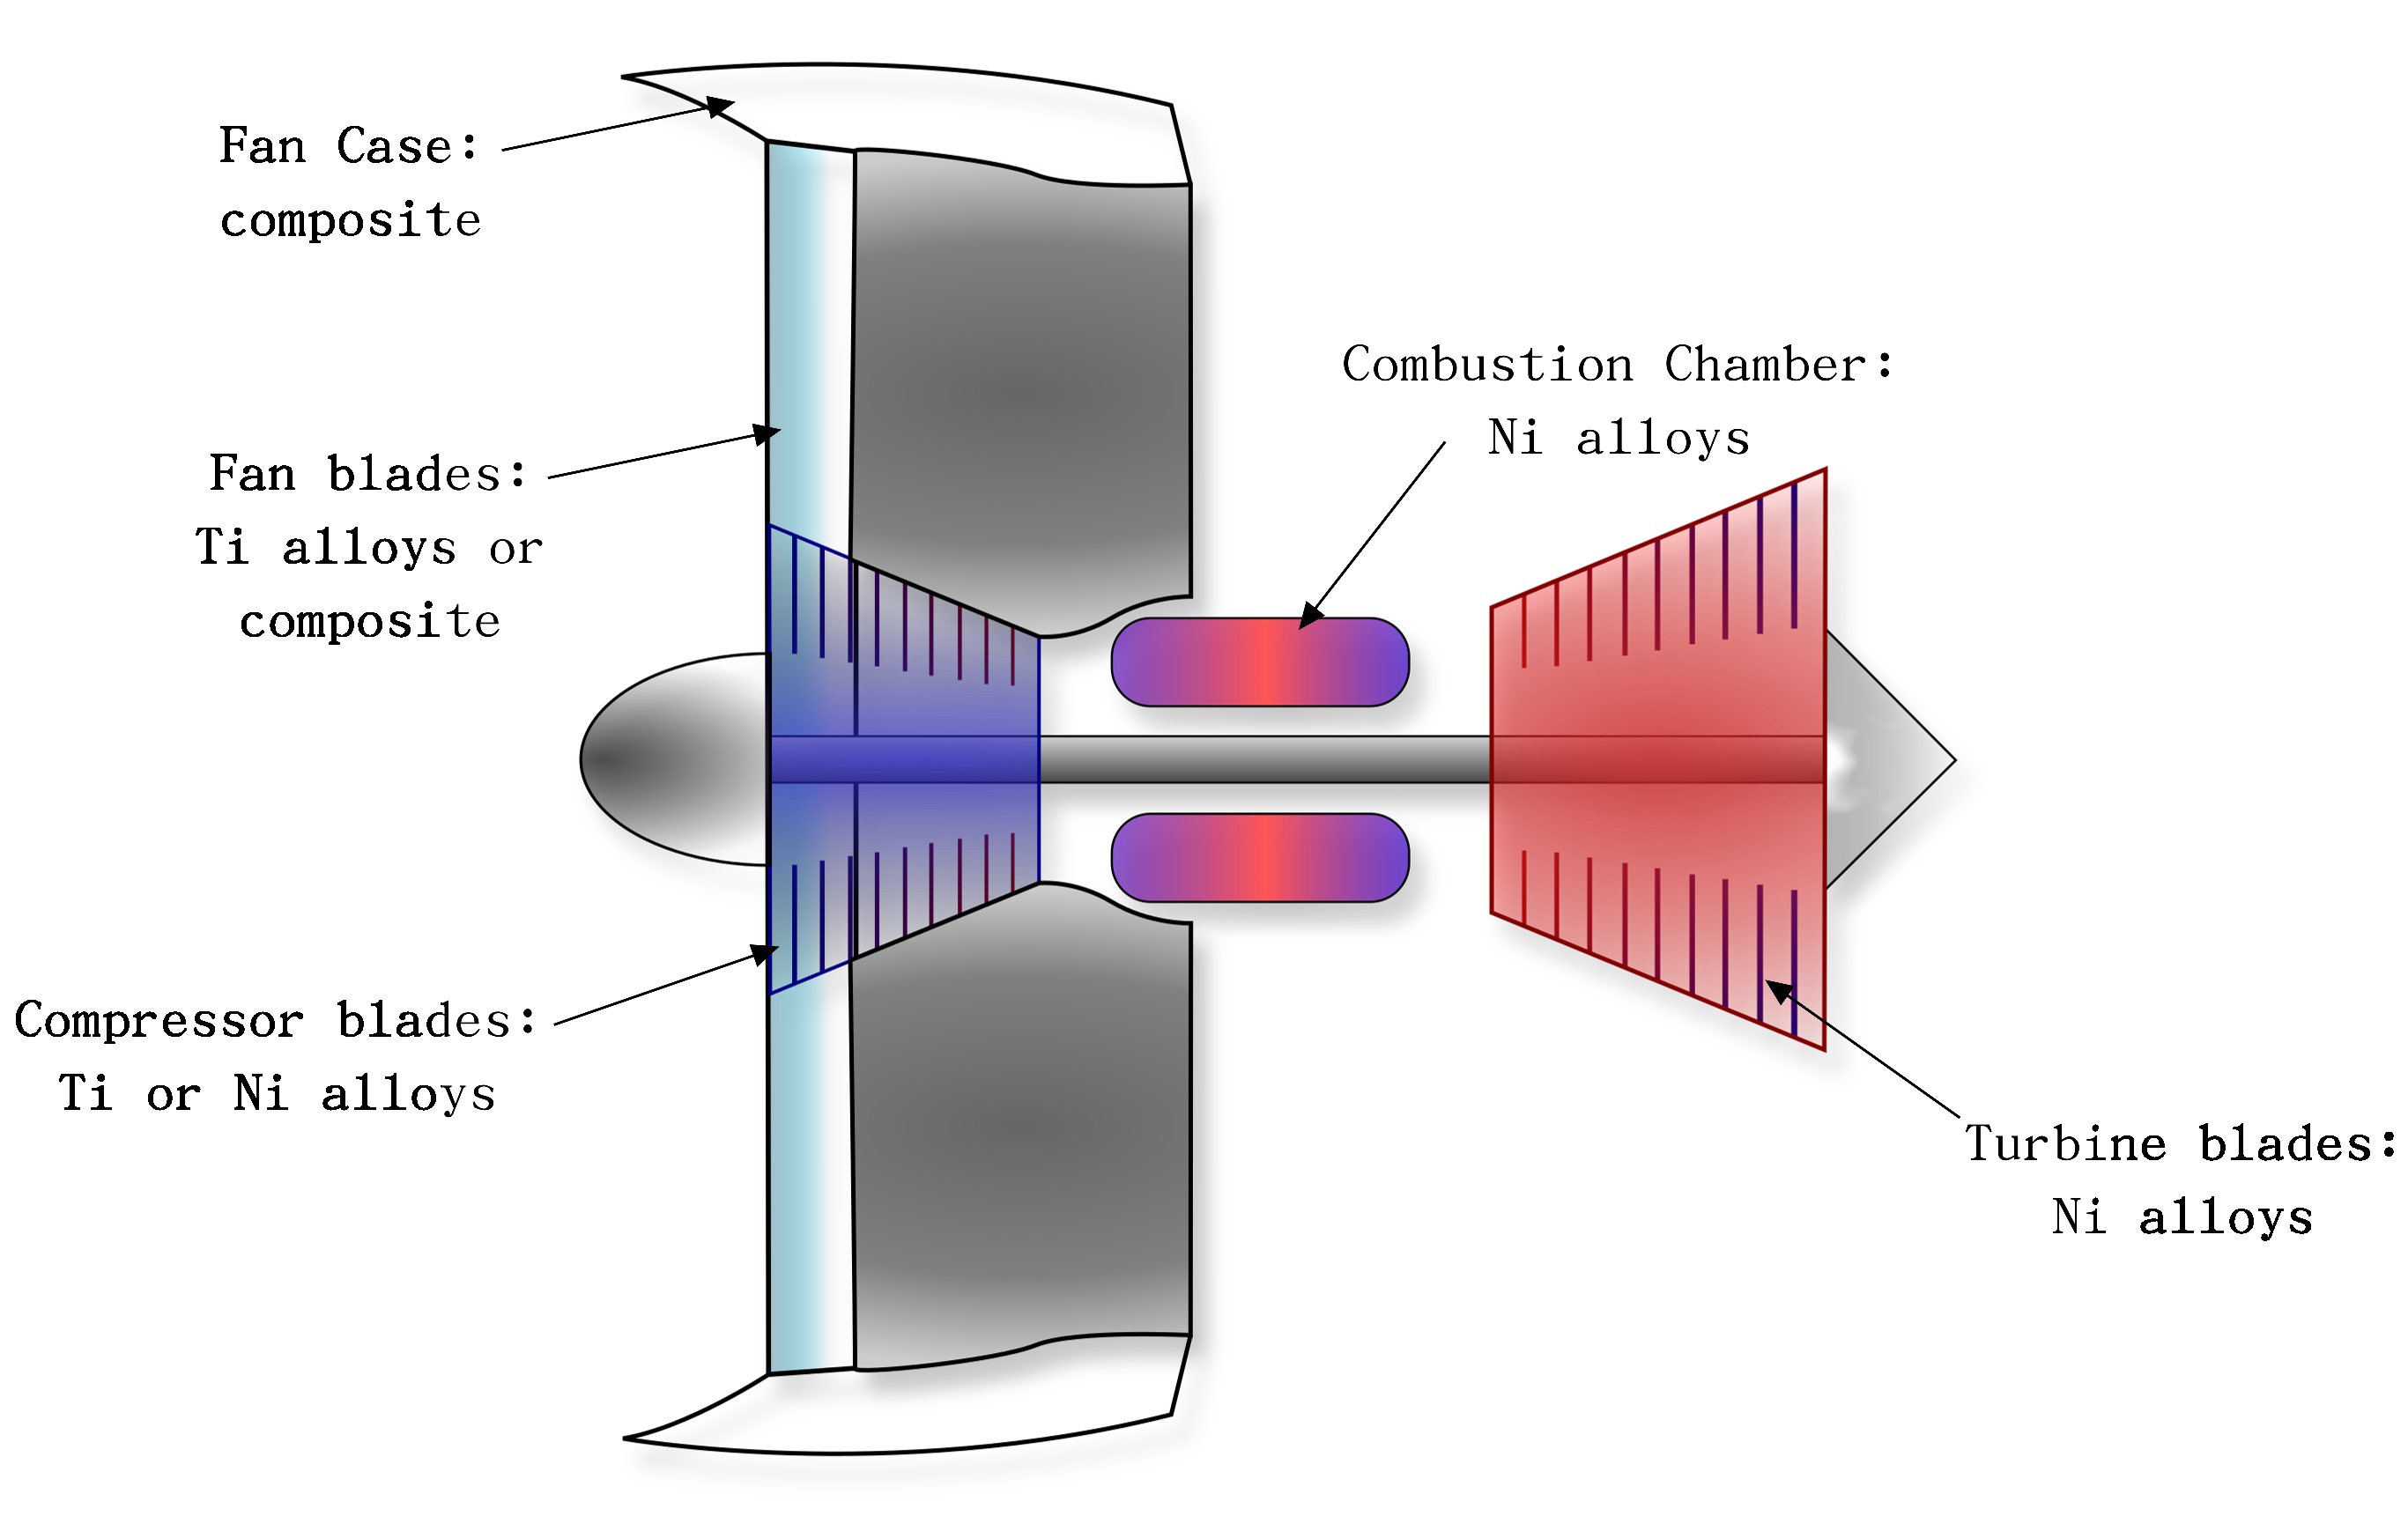
\includegraphics[width=0.9 \textwidth]{Sources/engine_drawing.eps}
        \caption{Materiali tipici in un motore turbofan \autocite{Inkscape}}
    \end{figure}

    Queste superleghe hanno portato innumerevoli benefici nell'efficienza operativa
    complessiva dei moderni velivoli.

    Ad esempio, all'aumentare del gradiente termico operativo, aumenta il rendimento del motore, 
    con un impatto positivo sull'efficienza e sui costi complessivi.

    Inoltre, l'elevata resistenza agli sforzi ciclici, a cui le palette sono 
    continuamente sottoposte, consente una riduzione e semplificazione delle invasive operazioni
    di manutenzione a terra, diminuendo quindi l'introduzione di errori umani e, allo stesso
    tempo, garantendo al velivolo un maggior numero di missioni durante la propria vita operativa.






    \clearpage

        \subsection{Composizione delle superleghe di Nickel\label{Nickel_composizione}}

        Una peculiaritá delle superleghe di Nickel é l'elevata presenza di elementi alliganti, fino 
        al 40-60\%, in una matrice di Nickel \autocite{Mouritz}. \\ 

        Sono tipicamente inseriti Cromo (10-20\%),
        Cobalto (5-15\%), Alluminio e Titanio (8\%, complessivamente), oltre
        a piccole quantitá di elementi
        come Molibdeno, Tungsteno e Carbonio. \\ \\ 

      
        \begin{table}[h!]
            \centering
            \resizebox{\textwidth}{!}{%
            \begin{tabular}{@{}cl@{}}
            \toprule
            \multicolumn{1}{l}{\textbf{Elemento}} & \textbf{Funzione}                                               \\ \midrule
            Cromo                                 & Rafforzamento per soluzione solida e resistenza alla corrosione \\
            Molibdeno                             & Rafforzamento per soluzione solida e resistenza al creep        \\
            Tungsteno                             & Rafforzamento per soluzione solida e resistenza al creep        \\
            Cobalto                               & Rafforzamento per soluzione solida                              \\
            Niobio                                & Indurimento da precipitati e resistenza al creep                \\
            Alluminio                             & Indurimento da precipitati e resistenza al creep                \\
            Carbonio                              & Tempra al carburo e resistenza al creep                         \\ \bottomrule
            \end{tabular}%
            }
            \caption{Funzione degli elementi alliganti \autocite{Mouritz}}
            \label{tab:funz_alliganti}
            \end{table}
        
        Nello specifico, le tre superleghe estrapolate dal database sono le seguenti:
        \textit{MAR-M 432, IN-162 e MAR-M 421}.

        Ulteriori criteri di selezione progettuale sono applicati in sezione \ref{material_index}.

    \clearpage

    \section{Processo Produttivo: Casting\label{Casting}}

    Negli ultimi anni, la manifattura additiva ha iniziato a soppiantare svariati 
    processi piú tradizionali, in primis nel settore aerospaziale. 

    In particolare, la capacitá di produrre geometrie complesse e non ottenibili
    con lavorazioni sottrattive, ha reso la manifattura additiva di notevole interesse 
    nella produzione di palette, in cui sono presenti svergolature studiate ad hoc, 
    oltre alla frequente necessitá di renderle cave per un eventuale raffreddamento attivo.

    Tipicamente, per le palette in superleghe, si utilizzano il 
    \textit{Selective Laser Melting} e l'\textit{Electron Beam Melting}.
    
    In particolare, la seconda tecnica presenta una maggiore efficienza, nonché un rateo
    produttivo superiore e una maggiore affinitá con metalli molto
    riflettivi, difficilmente lavorabili
    in SLM.
    
    Tale rateo produttivo, specialmente se si considera il miglioramento della tecnologia
    negli anni, puó compensare l'esorbitante costo iniziale dei macchinari EBM, che devono operare in vacuum
    e garantire una schermatura esterna dai raggi X potenzialmente prodotti, aumentando
    notevolmente la complessitá del processo e la manutenzione che ne deriva. \\ 

    Nonostante le potenzialitá dell'AM, per seguire un workflow compatibile col database di \textit{Granta}, si é optato
    per un altro processo produttivo piú tradizionale, il \textit{casting}. 

    \begin{figure}[h!]
        \centering
        \phantomsection \label{low_press_mold}
        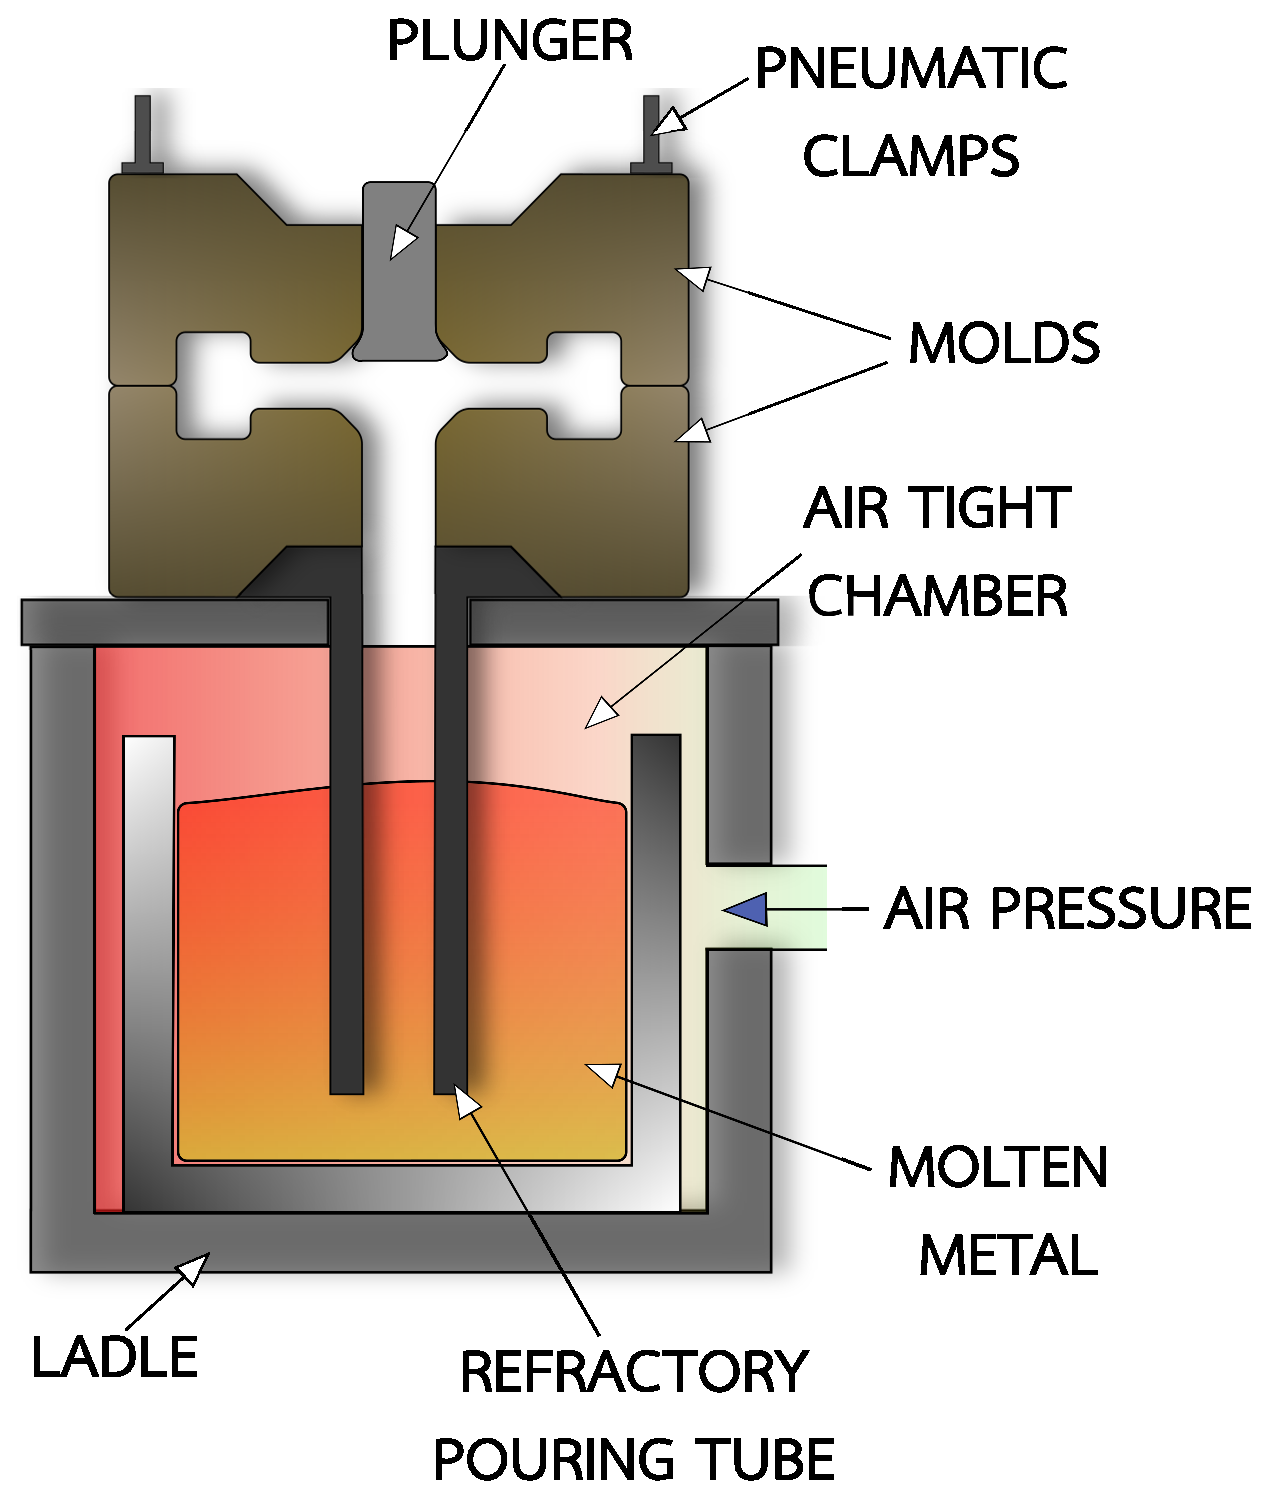
\includegraphics[width=0.45\textwidth]{Sources/pressurized_mold.eps}
        \caption{Schema di un casting in low-pressure permanent mold \autocite{Inkscape}}
    \end{figure}


    Tra i metodi tradizionali, questa tecnica produttiva, che consiste nella solidificazione di metallo fuso
    in uno stampo dalla geometria prossima a quella desiderata, si é notevolmente evoluta negli ultimi anni,
    al punto da essere il gold standard nella
    produzione di parti in superleghe di Nickel ad alte prestazioni, con tecniche avanzate come il casting con
    gas a bassa pressione o l' \textit{investment casting} in vacuum, scelta definitiva per la manifattura del componente. 

    Altri processi quali ad esempio il casting in lingotti, con successiva forgiatura o estrusione,
    portano troppo spesso a cricche e danni irreversibili durante la lavorazione, se applicati a queste superleghe \autocite{Mouritz}.

    Inoltre, seppur non sempre al livello della manifattura additiva, l'\textit{investment casting} consente comunque un minor spreco 
    di materiale, dato che le operazioni di natura strettamente sottrattiva sono limitate ad un'inevitabile
    rifinitura del componente estratto dallo stampo. \\ 

    Un altro vantaggio dell'\textit{investment casting}, decisivo nella scelta del processo
    produttivo (al momento della stesura di questa relazione), é il minor costo complessivo a fronte
    di un rateo di produzione molto alto. 

    Attualmente, infatti, la manifattura additiva é praticamente d'obbligo per geometrie estremamente complesse, 
    per le quali altri metodi sono inutilizzabili o troppo onerosi in termini di complessitá di progetto e di  
    di costi produttivi; inoltre, l'AM ha un notevole vantaggio economico nell'abbattimento iniziale dei costi.

    Tuttavia, allo stato attuale della tecnologia, la geometria di una paletta di turbina é realizzabile tramite
    \textit{investment casting}, che garantisce allo stesso tempo un abbattimento dei costi in una produzione
    su larga scala, come giá accennato.\\ 

    É peró doveroso far presente che, in un futuro sicuramente non molto lontano, i costi e la velocitá di manifattura
    dell'additive manufacturing su produzioni di massa saranno in grado di soppiantare definitivamente metodi piú tradizionali,
    anche in virtú del fatto che i brevetti su questa tecnologia sono scaduti nel 2016 \autocite{Latvian_additive}. 
    Molti gruppi di ricerca e grosse aziende del settore aerospaziale
    stanno infatti investendo continuamente sulla manifattura additiva,
    aprendo le porte anche a nuovi materiali e geometrie cave estremamente complesse, 
    generate automaticamente da calcoli strutturali con algoritmi di intelligenza artificiale, 
    con lo scopo di migliorare le prestazioni abbattendo allo stesso
    tempo la quantitá di materiale utlizzato e 
    cercando di rimpiazzare definitivamente il workflow della classica progettazione CAD, 
    intrinsecamente legata a processi di natura sottrattiva. \\ 

    Ulteriori considerazioni in merito all'AM sono presenti nella sezione \ref{conclusioni}.



    

    \clearpage

        \subsection{Solidificazione\label{Casting_solid}}

        Il principio alla base del casting é la solidificazione di un metallo fuso all'interno di uno
        stampo, la cui geometria verrá trasferita al prodotto finale, una volta estratto.

        Come per qualsiasi liquido, la condizione necessaria affinché
        avvenga tale passaggio di stato é il raffreddamento al di sotto della temperatura di solidificazione, 
        caratteristica di ogni materiale. 
        
        Questa condizione non é peró sufficiente: é infatti possibile che un liquido mantenga il suo 
        stato fisico per un tempo indefinito, anche molto al di sotto della temperatura di solidificazione, 
        nel fenomeno noto come \textit{supercooling}.

        Affinché avvenga la solidificazione, infatti, oltre al raggiungimento della temperatura target,
        é necessario che avvenga il fenomeno di \textit{nucleazione}. 

        Nel caso di un materiale puro (o molto vicino a tale condizione), nuclei identici, soggetti 
        ad un moto relativo sempre piú lento col decrescere della temperatura,
        cominciano a solidificare e a formare agglomerati policristallini di dimensione man mano crescente.

        Finché questi raggruppamenti di particelle solide non raggiungono una \
        \textit{dimensione critica}, in assenza di perturbazioni e di impuritá, i nuclei possono 
        ritornare in soluzione liquida; é per questo motivo che si verifica il supercooling.

        Una volta raggiunta tale dimensione critica, la solidificazione ha luogo per 
        \textit{nucleazione omogenea}.  

        Nel caso di materiali non puri, come ad esempio le leghe metalliche, il supercooling
        non si verifica poiché il sistema é ricco di molecole di vari altri materiali e impuritá, 
        che fungono da centro di nucleazione stabile. Anche le pareti di uno stampo, soprattutto 
        al crescere della superficie esposta, forniscono dei centri di nucleazione stabili. 

        Per questo motivo, nei materiali non puri avviene una \textit{nucleazione eterogenea}, 
        fenomeno che si instaura stabilmente e si autosostiene non appena si scende al di sotto della temperatura di 
        solidificazione \autocite{Mouritz}. \\ 

        Tale processo puó tuttavia essere studiato e controllato industrialmente al fine di 
        ottenere determinate proprietá meccaniche, fisiche e chimiche o anche estetiche nel prodotto finale, 
        manipolando vari parametri come la velocitá di raffreddamento o l'inserimento di percentuali
        variabili di elementi alliganti nelle leghe. 

        Tutti questi procedimenti, oltre ad eventuali trattamenti termici successivi, influenzano le 
        caratteristiche finali del prodotto, agendo sulla struttura cristallina del materiale e
        a tale scopo, si fa riferimento ai \textit{diagrammi di fase}.

            \begin{figure}[h!]
                \centering
                \phantomsection \label{fig:diagramma_fase}
                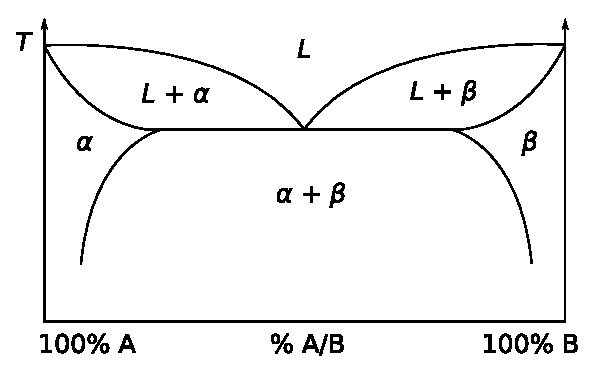
\includegraphics[width=0.3\textwidth]{diagramma_fase.eps}
                \caption{Diagramma di fase binario generico \autocite{phase_diagram_generic}}
            \end{figure}
        




        \clearpage
        \subsection{Struttura\label{Casting_strutt}}

            \subsubsection{Zone fredde, colonnari e centrali\label{Casting_strutt_zone}}

            \begin{figure}[h!]
                \centering
                \phantomsection \label{fig:grain_casting}
                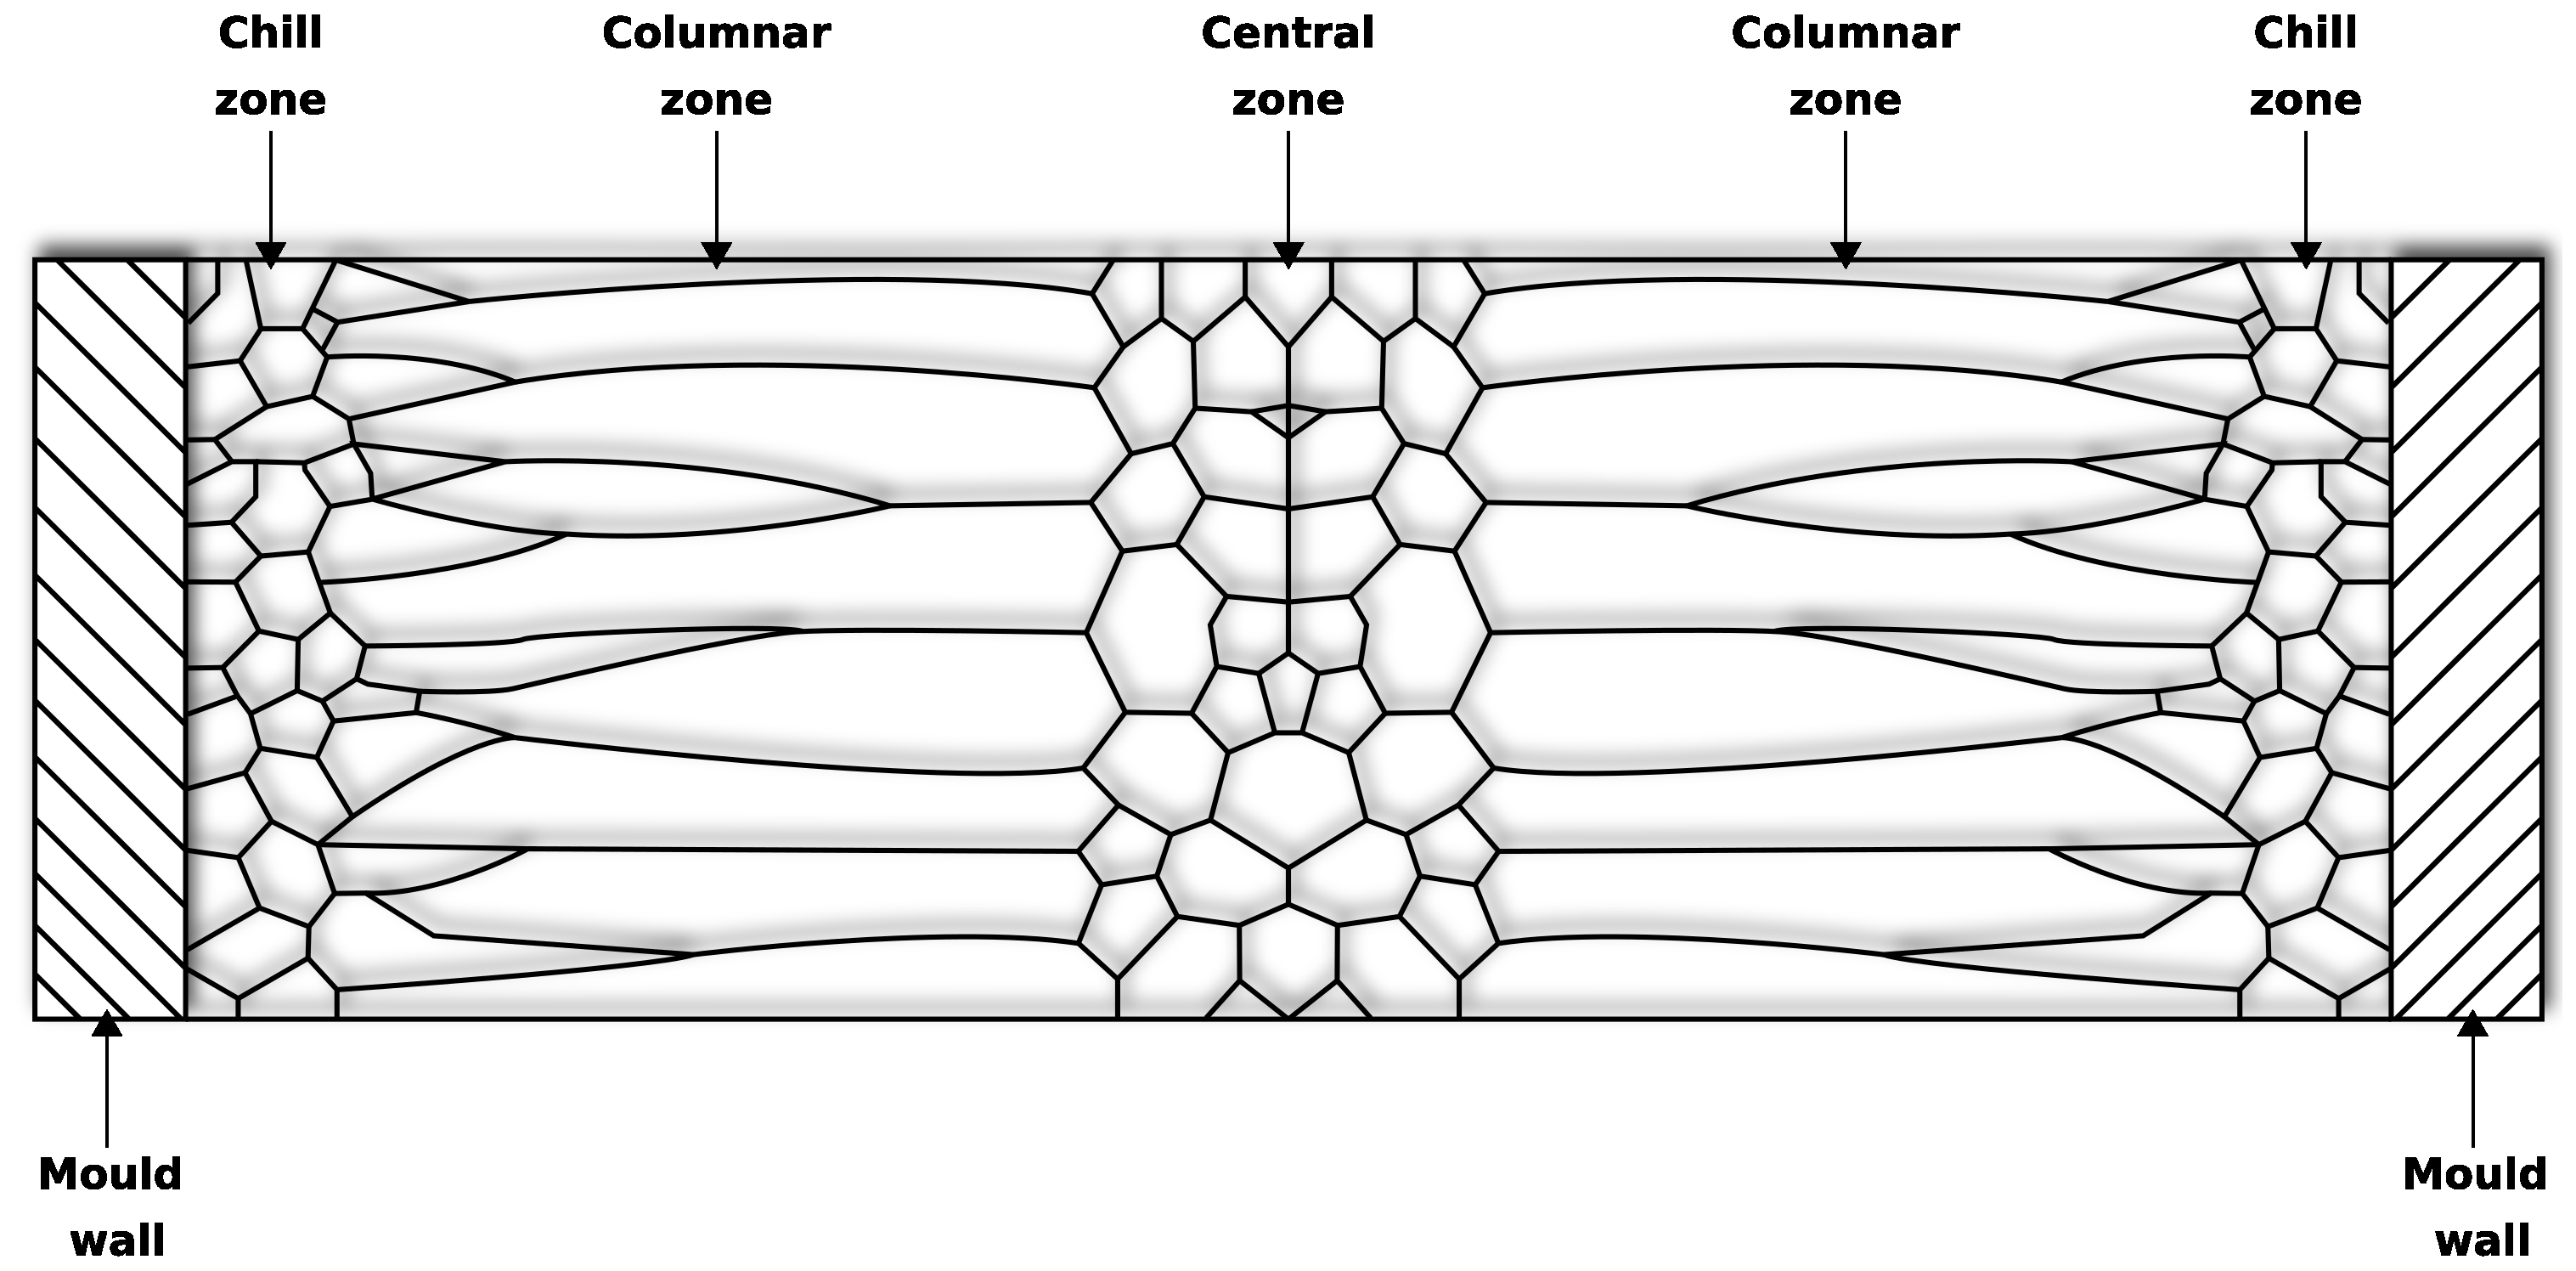
\includegraphics[width=\textwidth]{Sources/grain.eps}
                \caption{Grani di un lingotto raffreddato \autocite{Inkscape}}
            \end{figure}


            Considerando per semplicitá di esposizione lo stampo di un lingotto, in sezione si possono osservare
            delle macroaree distinte con struttura del grano differente. 
            
            Per una data composizione di una lega, la geometria, la dimensione e la disposizione caratteristica di tali grani dipendono fortemente, come giá
            accennato, dalla velocitá di raffreddamento, che a sua volta é influenzata dalla temperatura di colata, dalla forma 
            macroscopica dello stampo e quindi dal volume di metallo liquido che puó ospitare.

            Come si osserva in figura (\ref{fig:grain_casting}), le tre regioni distinte sono:

                \begin{itemize}
                    \item \textit{Zona fredda} \\ \\ 
                        Questa regione é la prima a formarsi, per nucleazione
                        eterogenea facilitata dal contatto con le pareti dello stampo, che oltretutto incrementano
                        la velocitá di raffreddamento locale del metallo.

                        I grani, che in questa zona si formano molto rapidamente, continuano ad incrementare
                        la propria dimensione finché non vengono ostacolati e vincolati dalla presenza degli altri grani adiacenti. 

                        Il grano si presenta dunque di forma irregolare ma non allungata e di dimensioni
                        consistenti, ed é distribuito tipicamente nell'intorno
                        delle pareti.

                        Tuttavia, nel caso di una temperatura di colata troppo bassa, la macrosolidificazione del 
                        lingotto avviene molto rapidamente, generando delle tensioni che fanno staccare i nuclei dalla 
                        zona fredda, i quali si distribuiscono piú omogeneamente in tutto il restante metallo liquido, 
                        fungendo a loro volta da centri di nucleazione e innestando un effetto a catena, che fa solidificare
                        tutto il metallo con una distribuzione di grano complessivamente uguale a quella della zona fredda: non
                        sono quindi apprezzabili altre zone distinte \autocite{Mouritz}.
                    \item \textit{Zona colonnare} \\ \\ 
                        Nella maggior parte dei casi, la temperatura di colata del casting viene mantenuta il piú elevata
                        possibile.

                        In seguito alla formazione della zona fredda, la zona colonnare inizia piú lentamente a formarsi a partire da essa.

                        É caratterizzata da grani di forma aciculare, a sviluppo medio ortogonale rispetto alle pareti dello
                        stampo e in direzione opposta al flusso di calore (dalle zone piú fredde a quelle piú calde);
                        lo sviluppo segue inoltre la direzione energeticamente piú favorevole \autocite{Mouritz}.

                    \item \textit{Zona centrale} \\ \\ 
                        In alcuni casi, il metallo continua a solidificarsi seguendo lo sviluppo colonnare.

                        Tuttavia, il piú delle volte, si sviluppa indipendentemente una zona centrale equiassiale,
                        con grani relativamente piú tondeggianti rispetto alla zona fredda e di orientamento casuale.

                        Questi grani bloccano la crescita della zona colonnare quando vi entrano in contatto.

                        La prevalenza complessiva di zona centrale o di zona colonnare dipende dal gradiente termico tra l'interfaccia 
                        solido-liquido, legato, oltre che al materiale stesso, anche alla forma dello stampo e al volume
                        di liquido che quindi puó ospitare.

                        Piú é basso il gradiente termico, piú viene favorito il sopravvento della zona equiassiale. Viceversa, 
                        un forte gradiente termico fa prevalere la formazione di grani colonnari \autocite{Mouritz}.
                \end{itemize}

            \clearpage 



        \subsection{Difetti\label{Casting_difetti}}

        Nel settore aerospaziale, le normative in merito alla produzione di componenti per velivoli, in Europa
        regolate dall'\textit{EASA}, prevedono controlli molto piú stringenti rispetto ad altri settori 
        come quello automobilistico. 

        Molto spesso addirittura non si effettuano controlli a campione su un lotto di produzione, ma si 
        procede al controllo per ogni singolo componente. 

        In particolare, nel casting non devono essere presenti difetti che compromettano l'integritá
        strutturale del componente, per cui si attuano controlli severi in merito alla porositá, al ritiro, 
        alla presenza e distribuzione di inclusioni intermetalliche e alla segregazione di elementi di lega.
 

            \subsubsection{Porositá e ritiro\label{Casting_difetti_porosita}}

            La formazione di pori é dovuta alla presenza di gas rimasti intrappolati all'interno del materiale, 
            durante la solidificazione.

            Possono presentarsi pori di forma irregolare oppure \textit{wormholes}, ossia pori di forma tubolare, 
            formati a causa dell'espansione forzata di bolle d'aria nella direzione del flusso di calore.
            
            Altre bolle d'aria possono formarsi a causa del ritiro del metallo durante la solidificazione.

            In ogni caso, la porositá compromette l'integritá strutturale del componente. 
            Si puó eliminare la porositá di un materiale sottoponendolo ad un trattamento termico noto come
            \textit{Hot Isostatic Pressing}, che consiste nell'esposizione ad alta temperatura e alta pressione, 
            in una camera con un gas inerte. 

            Tale processo consente l'eliminazione di cavitá e microporositá attraverso l'effetto combinato 
            di deformazione plastica, creep e diffusione allo stato solido, garantendo al componente, tra i vari benefici,
            una maggiore \textit{resist fatigue} \autocite{Mouritz}.


            \subsubsection{Inclusioni\label{Casting_difetti_inclusioni}}

            Durante la solidificazione, a seconda delle condizioni di raffreddamento 
             descritte 
            dal diagramma di fase opportuno, si ottengono per precipitazione dei composti intermetallici, 
            che formano delle inclusioni, spesso causa di frattura del componente.  

            Infatti, tali inclusioni interagiscono con le dislocazioni e causano la crescita di microcavitá interne, 
            che si uniscono in una cricca centrale, su un piano perpendicolare alla retta d'azione
            del carico sollecitante. 

            Durante questa fase, nei materiali come le leghe metalliche, si ha un accumulo di energia di 
            deformazione plastica, fino al raggiungimento di una dimensione critica della macrocricca, oltre il quale
            si verifica la frattura duttile. 

            Proprio nel caso dei materiali duttili, lo stress che porta a rottura il materiale puó essere
            sostanzialmente inferiore alla \textit{ultimate tensile strength}. Questo si rivela un problema 
            anche su lunghe scale di tempo, in cui un componente é sottoposto a sollecitazioni cicliche di bassa
            entitá, durante le quali avviene peró la propagazione di cricche, per le quali le inclusioni
            fungono da punto di concentrazione di stress. 

            Inoltre, le inclusioni presentano coefficienti di espansione termica considerevolmente differenti
             da quelli del materiale
            dominante, in quanto composti intermetallici. 

            Questa differenza porta a ulteriori concentrazioni di stress localizzati nell'intorno
            dell'inclusione.

            É quindi fondamentale controllare il processo di solidificazione seguendo i diagrammi di fase, 
            tenendo conto che la formazione di precipitati intermetallici é influenzata dalla velocitá
            di raffreddamento ma anche dalla percentuale e dal tipo di elementi alliganti inclusi nella lega, 
            che possono essere manipolati a seconda delle esigenze \autocite{Mouritz}. 

            \subsubsection{Segregazione degli elementi di lega\label{Casting_difetti_segregazione}}

            La solidificazione di una lega metallica comporta inevitabilmente una distribuzione non esattamente 
            omogenea degli elementi che la compongono, che possono quindi trovarsi segregati in zone di discontinuitá. \\ 

            Tale fenomeno si puó manifestare come \textit{macrosegregazione} se coinvolge l'intero 
            componente su larga scala ed é legato al gradiente termico tra zone superficiali e zone
            centrali, per le quali si instaura un rateo di diffusione molto differente. 

            Questo porta ad una forte anisotropia del componente, che presenta appunto proprietá 
            fisiche variabili tra il centro e la superficie. \\ 

            Se invece il fenomeno si manifesta su una scala inferiore alla dimensione media del grano, 
            prende il nome di \textit{microsegregazione} ed é dovuto alla differenza di composizione locale
            del nucleo dendritico, che é piú ricco di elementi alliganti al centro in cui comincia la nucleazione. \\ 

            La segregazione puó essere mitigata o del tutto risolta attraverso trattamenti termici prolungati ad alta temperatura,
            tipicamente poco sotto il punto di fusione. 

            Le elevate temperature, se protratte per un tempo sufficientemente lungo, favoriscono la diffusione
            molecolare, permettendo quindi ai vari elementi di distribuirsi in maniera piú omogenea nel componente \autocite{Mouritz}. 


    
            \clearpage

        \subsection{Investment casting\label{Casting_investment}}

        Come giá accennato all'inizio in sezione \ref{Casting}, esistono numerose tecniche 
        appartenenti alla famiglia del casting, un processo produttivo giá utilizzato da millenni 
        e dalle piú disparate civiltá. \\ 

        Senz'ombra di dubbio, tra le notevoli evoluzioni di questa tecnica nel corso della storia, l'
        \textit{investment casting} si presta in maniera eccezionale alla produzione di componenti
        dalle geometrie complesse, con tolleranze piú strette e finiture superficiali molto fini, 
        al punto da essere al momento il gold standard per la produzione di palette di turbina. \\

        La tecnica prevede l'utilizzo di un modello sacrificale della geometria
        finale, realizzato in un materiale a basso costo, come
        una cera, una resina o una schiuma, attorno al quale viene poi formato il vero e proprio stampo, 
        tipicamente in materiali refrattari in grado di ospitare il metallo fuso.

        É sufficiente poi far sciogliere il modello iniziale per ottenere lo stampo entro cui 
        viene versato il metallo \autocite{Mouritz}.

        L'investment casting esiste sin dall'antichitá e al giorno d'oggi si realizza con
        tecniche e macchinari molto piú sofisticati, che tipicamente rappresentano la barriera di costo
        iniziale, da ammortizzare nel tempo con un alto rateo di produzione.  \\ 

        Oltre al pouring per effetto della gravitá, nella 
        produzione di componenti ad 
        elevate prestazioni, si utilizzano tecniche piú avanzate come il 
        \textit{vacuum casting}, in cui un vuoto risucchia nella cavitá
        il materiale fuso, attraverso un condotto, in direzione opposta alla gravitá. 

        Una volta solidificata la quantitá di materiale necessario attorno alle pareti,
        viene rilasciato il vuoto, permettendo al metallo in eccesso di fluire via ed essere riutilizzato. \\ 


        Attualmente, come giá ribadito piú volte, l'\textit{additive manufacturing} si sta rivelando
        man mano sempre piú competitivo col casting, per quanto detto all'inizio in sezione \ref{Casting}. 

        Ció non vuol dire che le due tecniche debbano necessariamente essere in antitesi l'una con l'altra, é 
        infatti oggi molto comune utilizzare la manifattura additiva per produrre le componenti in resine 
        destinate alla creazione degli stampi da investment casting, anche nello specifico per quanto riguarda la produzione
        di palette. 


        \clearpage


    \section{Indici di merito\label{material_index}}


        Una buona strategia di analisi qualitativa per la selezione di materiali é rappresentata dalla valutazione di alcuni parametri frazionari, riferiti a una moltitudine di proprietá fisiche, chimiche, termiche, meccaniche, ecc, noti come indici di merito.
        
        Tali indici, definiti ad hoc in base alle necessitá del progettista, consentono di effettuare rapidamente un’indagine comparativa tra una lista di potenziali candidati che hanno superato una fase di preselezione, nel caso in cui la scelta del materiale non sia particolarmente ovvia o scontata. 
        \\ \\
        Nel caso specifico della paletta di uno stadio di turbina ad alta pressione, come piú volte ribadito, sorgono diverse sfide con requisiti estremi da soddisfare simultaneamente.

        Possono quindi tornare molto utili alcuni indici di merito, dato che devono essere garantiti una elevata temperatura di esercizio, un basso coefficiente di espansione termica, un’alta fracture toughness, un’alta resistenza a fatica, un elevato modulo elastico, un’alta frequenza naturale di risonanza, oltre che un’ottima resistenza all’aggressivitá chimica dell’ambiente operativo. 
        
        Tutti i possibili indici di merito di un materiale sono spesso definiti in funzione della densitá, specialmente in campo aerospaziale, in cui l’ottimizzazione del peso di ogni componente risulta fondamentale, tra le svariate motivazioni, per massimizzare l’efficienza propulsiva, riducendo quindi la spesa sul carburante, che ha un impatto sostanziale sui costi complessivi di un velivolo e sulla sostenibilitá \autocite{EASA_environ_report_2019}.
        \\ \\ 
        In seguito alla promettente fase di preselezione sul database,
        superata da tre materiali candidati, si é deciso di concentrarsi sugli indici relativi alla \textit{fracture toughness} e alla \textit{resist fatigue},
        per le quali i materiali preselezionati non mostrano evidenti compromessi ottimali.

        \begin{figure}[h!]
            \centering
            \phantomsection \label{blade_load}
            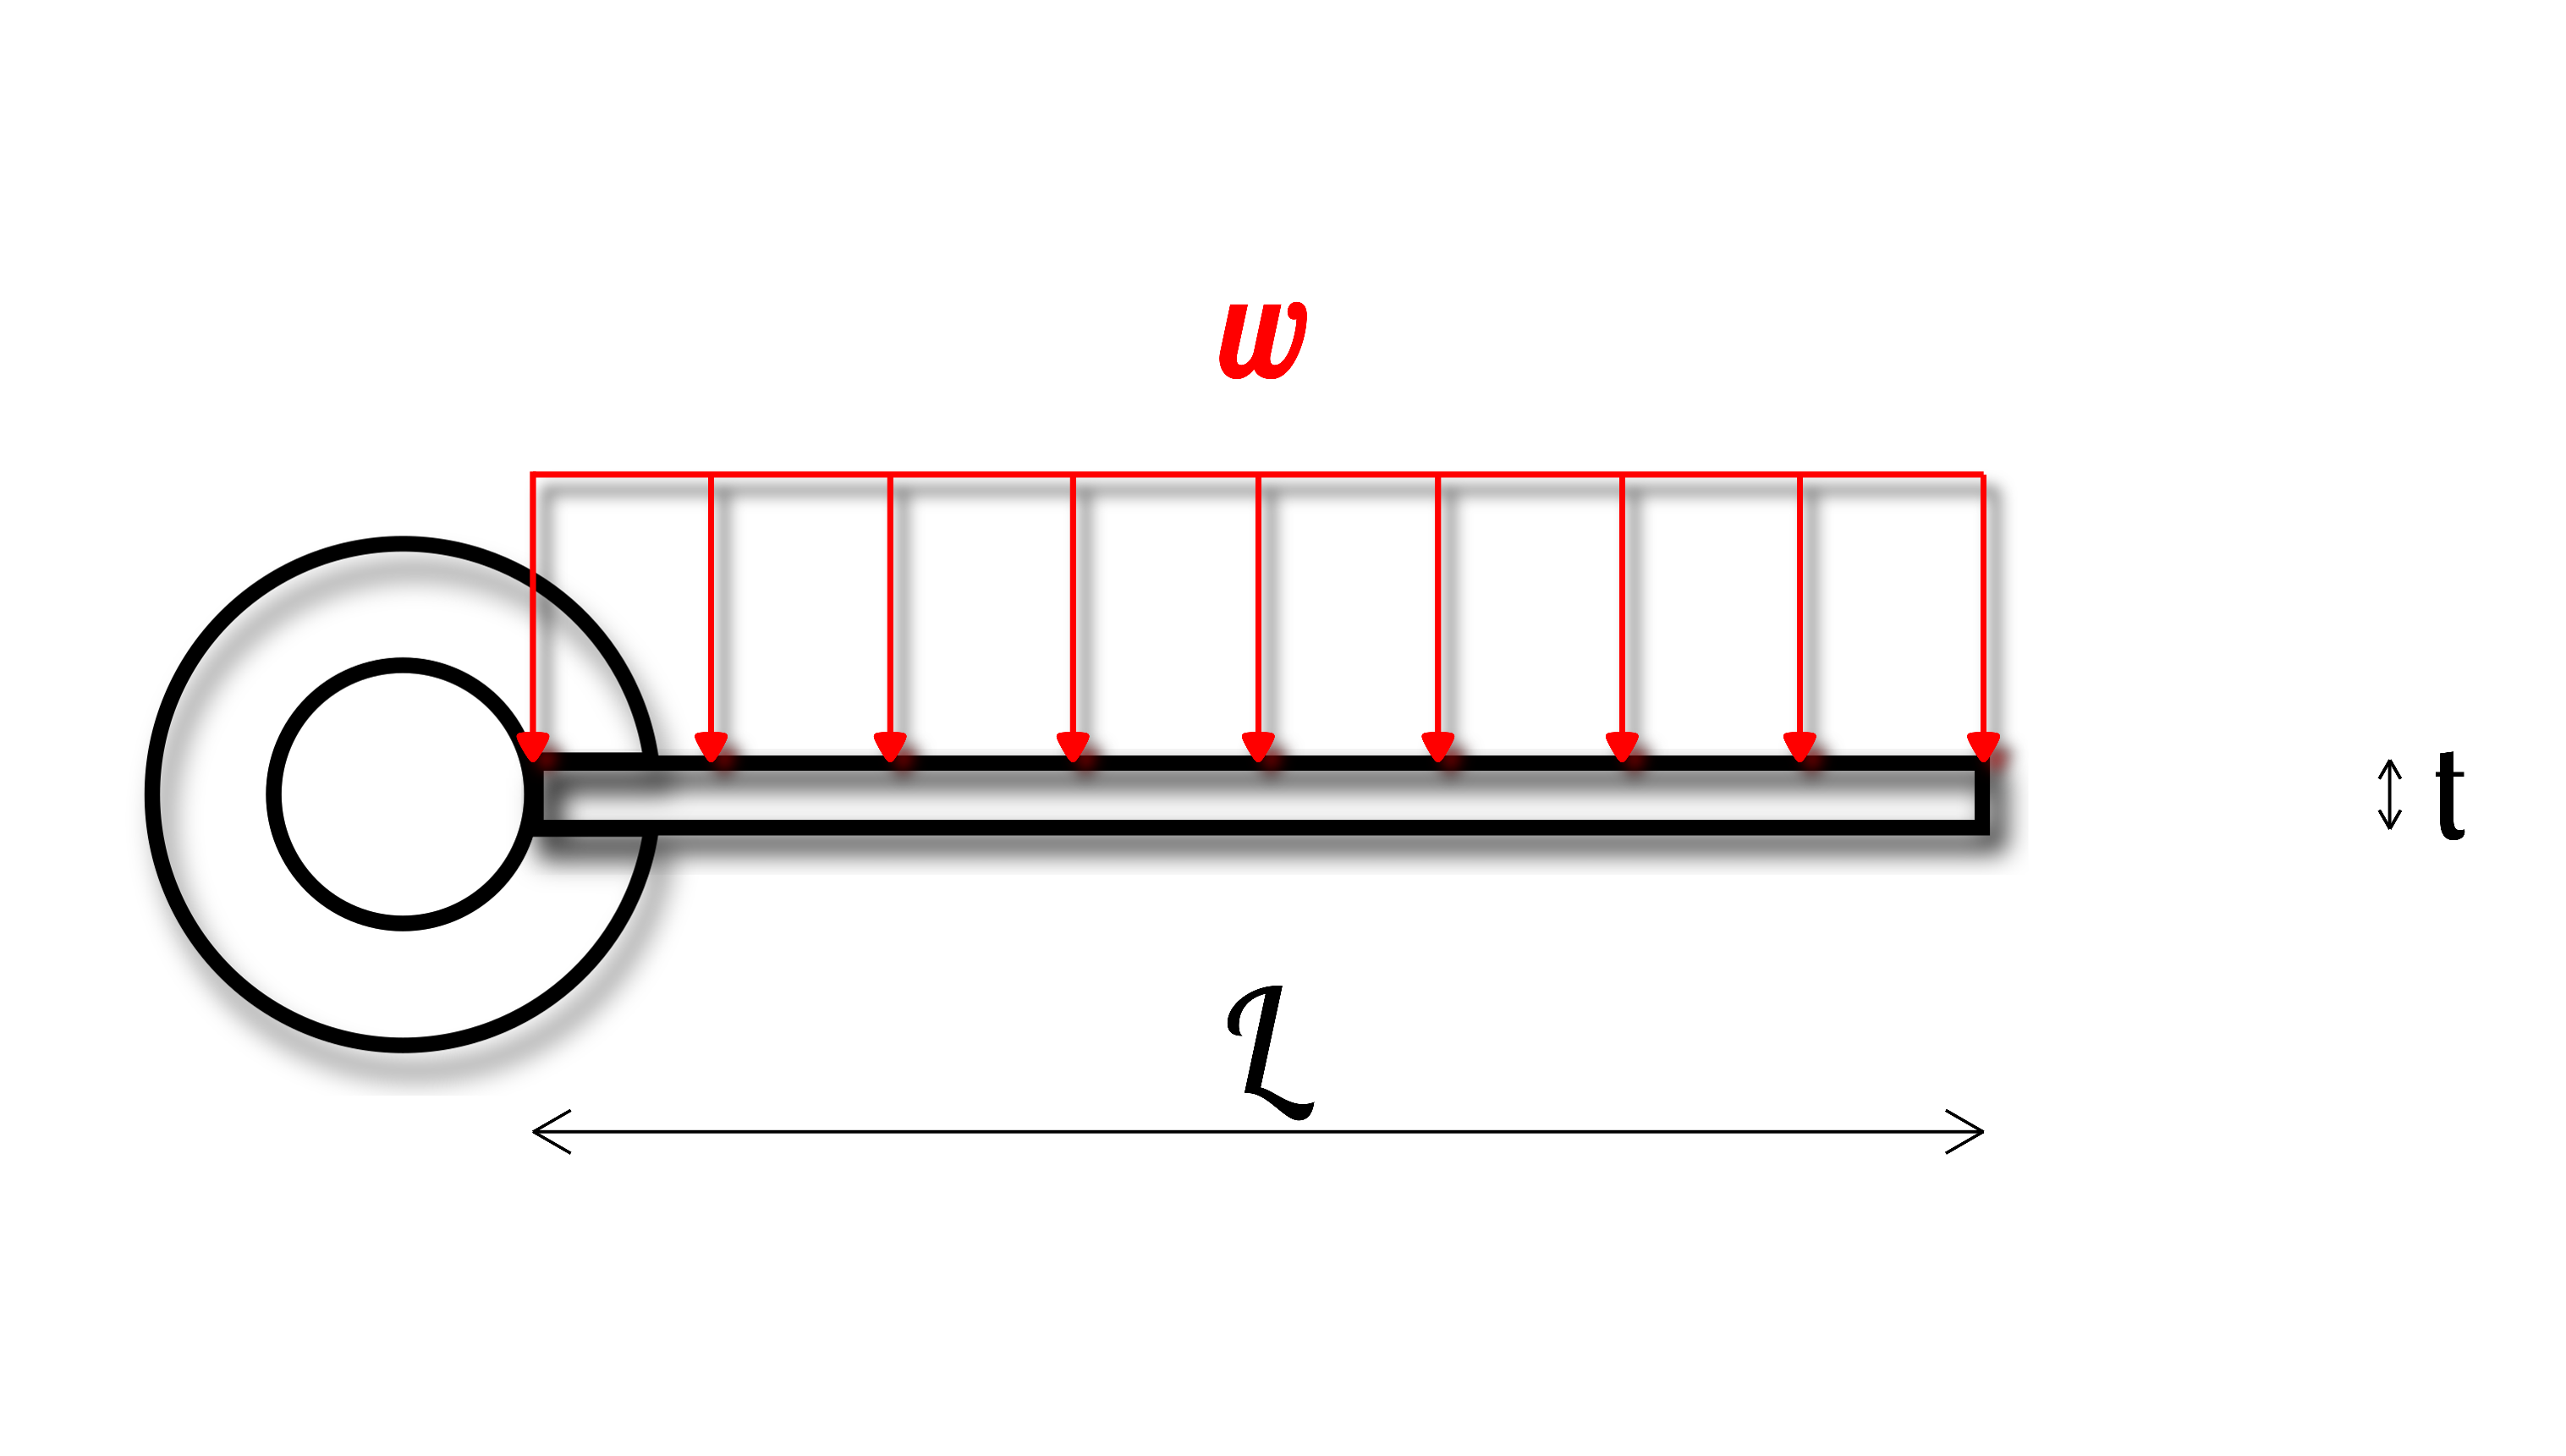
\includegraphics[width=0.8\textwidth]{Sources/blade_load.eps}
            \caption{Schematizzazione semplificata di una paletta \autocite{Inkscape}}
        \end{figure}
        \clearpage

        Per semplificare i calcoli, si assume una paletta rappresentata da una trave a base rettangolare
        estrusa, caratterizzata da:

        \begin{itemize}
            \item Lunghezza \textit{L} [m]
            \item Spessore \textit{t} [m]
            \item Larghezza $\lambda t \ [m]$ (con aspect ratio $\lambda$)
            \item Carico uniformemente distribuito $w = \frac{F}{L}$ [N/m]
            \item Stress applicato $\sigma(y) = \frac{M}{I} \cdot y \ \ \ [\frac{N}{m^2}]$ (dall'equazione di \textit{Navier})
                \begin{itemize}
                    \item $I = \frac{\alpha t^4}{12} \ \ [m^4]$ 
                    \item $M = \frac{wl^2}{2} \ \ [N \cdot m]$
                \end{itemize}
            \item Stress massimo per $\sigma_{max} = \sigma(y = \frac{t}{2})$
            \item Area della sezione $A = \lambda t^2 \ [m^2]$
            \item Densitá $\rho \ [\frac{kg}{m^3}]$
            \item Massa $m = \rho \cdot AL \ \ [kg]$
        \end{itemize}

        Attraverso una manipolazione delle giuste grandezze, gli indici di merito di interesse possono essere ricavati 
        in maniera del tutto indipendente dalla geometria della paletta, focalizzandosi quindi
        sulle proprietá intrinseche del materiale.
        \\ \\ 
        Ipotizzando che la paletta abbia una cricca centrale di dimensioni trascurabili
        rispetto alla sua larghezza, si definisce la \textit{fracture toughness}:

        \begin{equation}
            K_{1c} = \sigma\left(\pi c\right)^{0.5} 
            \phantomsection \label{equation:frac_tough}
        \end{equation}
        dove $\sigma$ é lo sforzo applicato, c é la dimensione della cricca. \\ \\ 

        Manipolando l'equazione con le caratteristiche della paletta precedentemente
        elencate, si ottiene una massa $m \propto \left(\frac{\rho}{K_{1c}}\right) $.

        Alla luce di quanto detto, si definisce il relativo indice di merito, da massimizzare \autocite{SciencePubGroup}:

        \begin{equation}
            i_{K} = \left (\frac{K_{1c}}{\rho}\right)
            \phantomsection \label{equation:index_frac_tough}
        \end{equation}
        \clearpage 

        Si procede in maniera del tutto analoga per definire un indice di merito relativo alla 
        \textit{resist fatigue}.

        Si definisce una \textit{resist fatigue} (che deve essere il piú alta possibile,
        visto l'onere delle sollecitazioni cicliche a cui é tipicamente sottoposta una paletta di turbina), 
        attraverso la disuguaglianza:

        \begin{equation}
            \sigma_e \geq \frac{wL}{A}
            \phantomsection \label{equation:resist_fatigue}
        \end{equation}

        Dopo varie sostituzioni algebriche, si ottiene una massa $m \propto \frac{\rho}{\sigma_e}$.

        Per cui in definitiva, si definisce il relativo indice di merito, da massimizzare \autocite{SciencePubGroup}:

        \begin{equation}
            \phantomsection \label{equation:resist_fatigue_index}
            i_{sigma} = \left (\frac{\sigma_e}{\rho}\right)
        \end{equation}

        Sfruttando queste definizioni ed i dati reperiti su \textit{Granta}, 
        sono stati calcolati i due indici di merito per ogni materiale, tramite un breve script in 
        \textit{Octave} \autocite{Octave}, disponibile nel repository di questo progetto \autocite{Relazione_materiali}. \\ 

        Considerando che, per come sono stati definiti, tali indici devono essere massimizzati al fine di ridurre il peso, 
        una possibile opzione é quella di comparare il valore massimo di ognuno dei due indici e trovare un compromesso
        a seconda delle prioritá di progetto.

        \begin{equation}
            Materials = [MARM432, \ IN162, \ MARM421] 
            \phantomsection \label{vector:material_list}
        \end{equation}

        \begin{equation}
            \vec{i}_{sigma} = [\textbf{0.0069325}, \  0.0053870, \  0.0060681
            ]
            \phantomsection \label{vector:index_fatigue}
        \end{equation}

        \begin{equation}
            \vec{i}_{K} = [0.00046442, \  \textbf{0.00055294}, \  0.00039814]
            \phantomsection \label{vector:index_frac_tough}
        \end{equation}

        Da (\ref{vector:material_list}), (\ref{vector:index_fatigue}) e (\ref{vector:index_frac_tough}) si evince come 
        la lega \textit{MARM432} presenti la migliore resistenza a fatica a paritá di peso, permettendo, potenzialmente, 
        una maggiore durata dell'operativitá del componente.

        D'altro canto, si evince anche che la lega \textit{IN162} ha una migliore fracture toughness a paritá di peso. 

        
            \begin{figure}[h!]
                \phantomsection \label{fig:indici_retta_frac}
                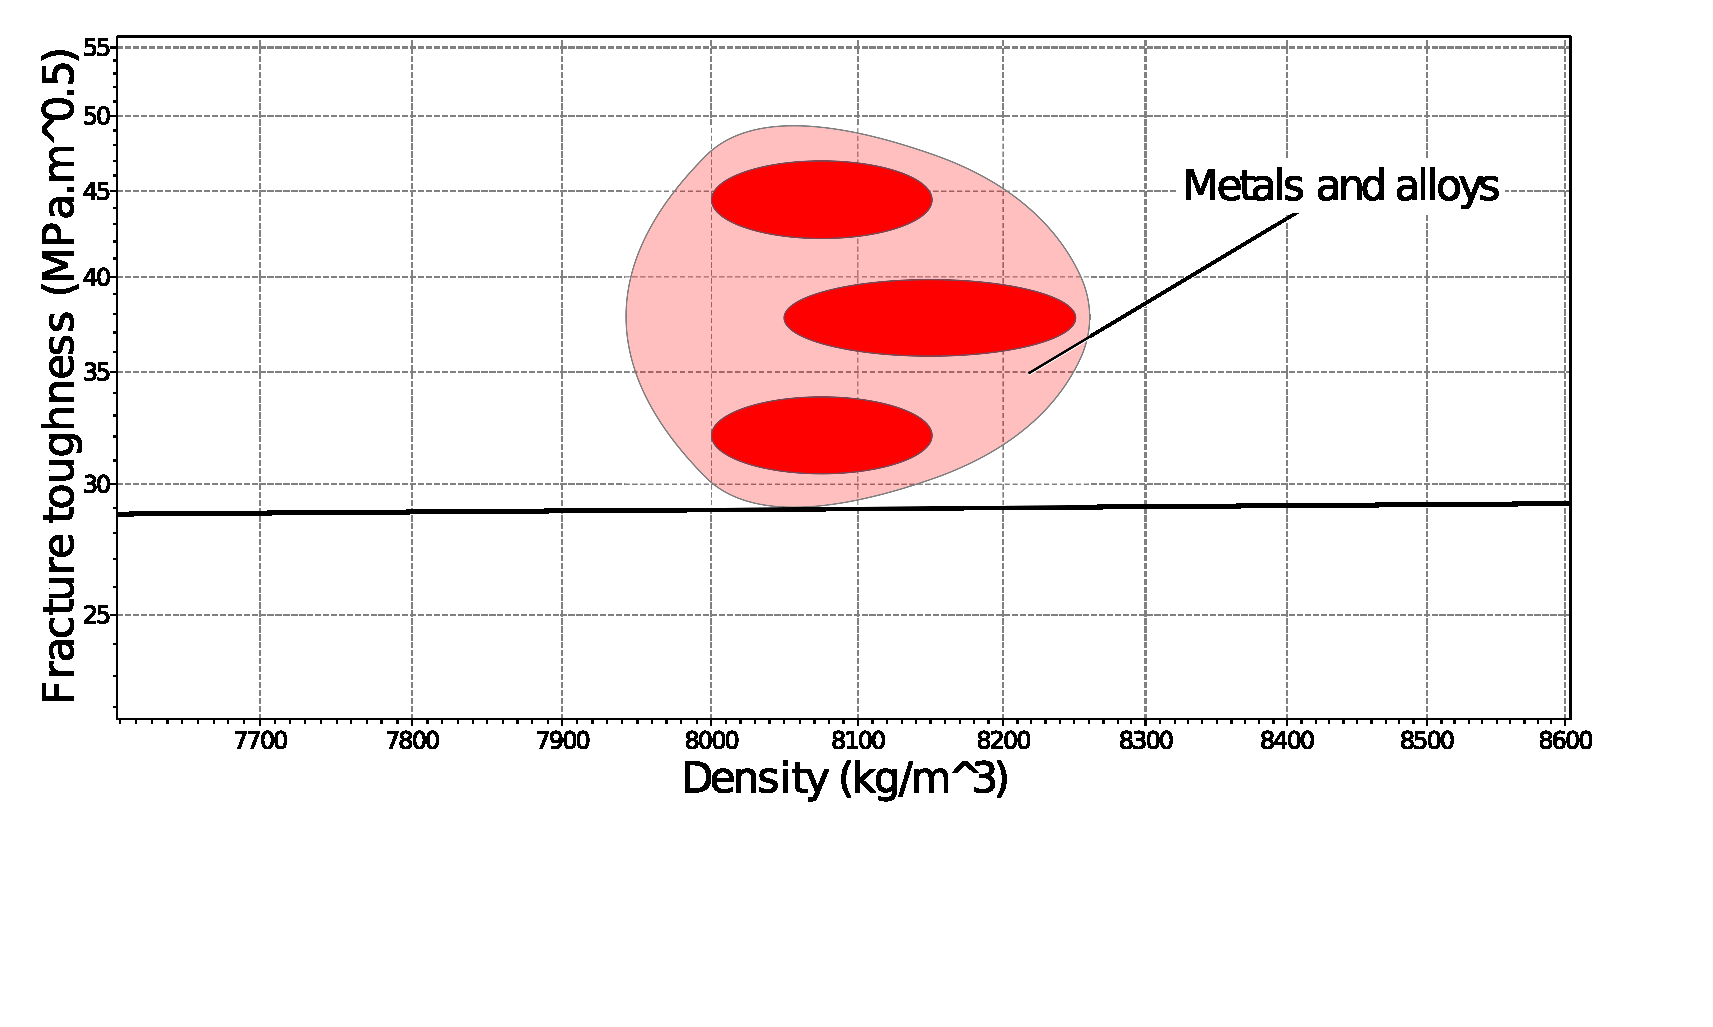
\includegraphics[width=\textwidth]{retta_frac.eps}
                \caption{Indice di merito rappresentato dalla pendenza della retta}
            \end{figure}

            \begin{figure}[h!]
                \phantomsection \label{fig:indici_retta_fatigue}
                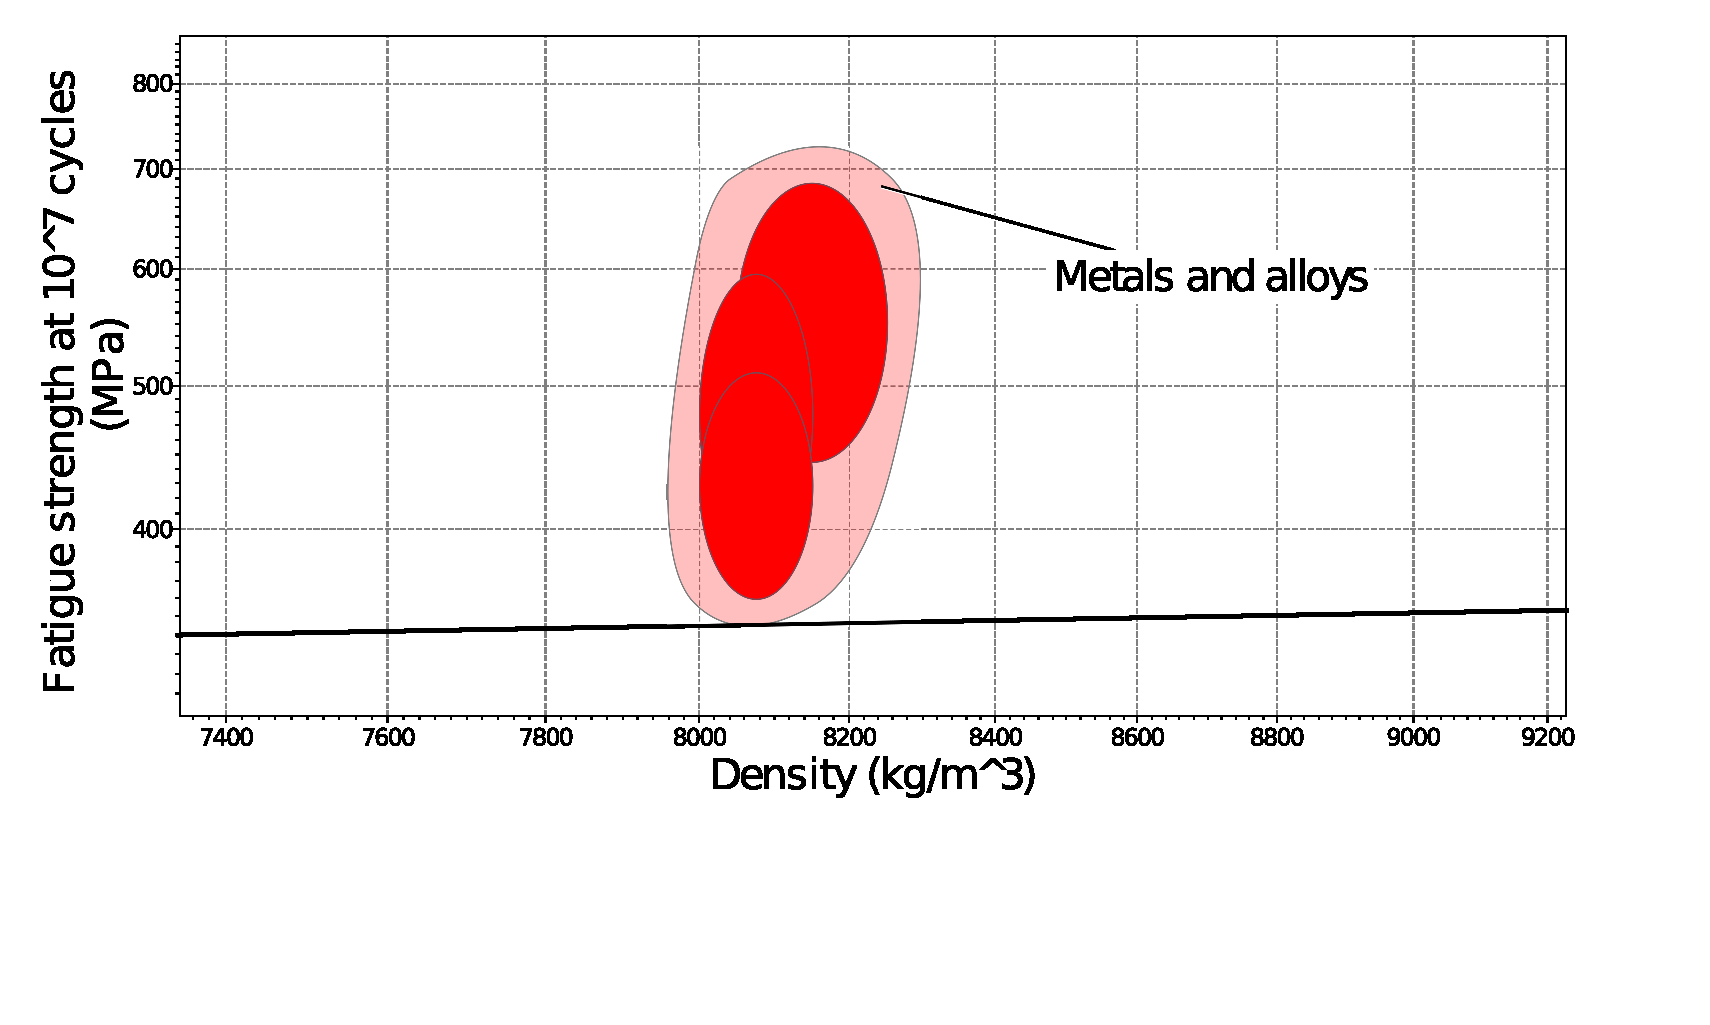
\includegraphics[width=\textwidth]{retta_fatigue.eps}
                \caption{Indice di merito rappresentato dalla pendenza della retta}
            \end{figure}

        \clearpage


    \section{Conclusioni\label{conclusioni}}

    \subsection{Scelta finale \label{scelta_finale}}

    É evidente come, tra i tre candidati, spicchino  in particolare \textit{MARM-432} e \textit{IN-162}, 
    ognuno per due proprietá diverse, anche se é doveroso mettere in risalto che tutti e tre i materiali
    non presentano differenze enormi nelle proprietá ritenute di interesse per questo progetto.
    
    Nel contesto di una produzione reale, potrebbero potenzialmente entrare in gioco altri fattori determinanti come
    la disponibilitá sul mercato, contatti giá consolidati con fornitori che producono un materiale piuttosto 
    che un altro, indici di costo (per quanto questi ultimi meno rilevanti nel settore aerospaziale), ecc. \\ 

    In questo caso, la scelta finale é stata determinata da considerazioni puramente prestazionali, rispetto 
    ai vincoli di progetto e agli indici di merito imposti. 

        \begin{figure}[h!]
            \phantomsection \label{fig:indici_di_merito}
            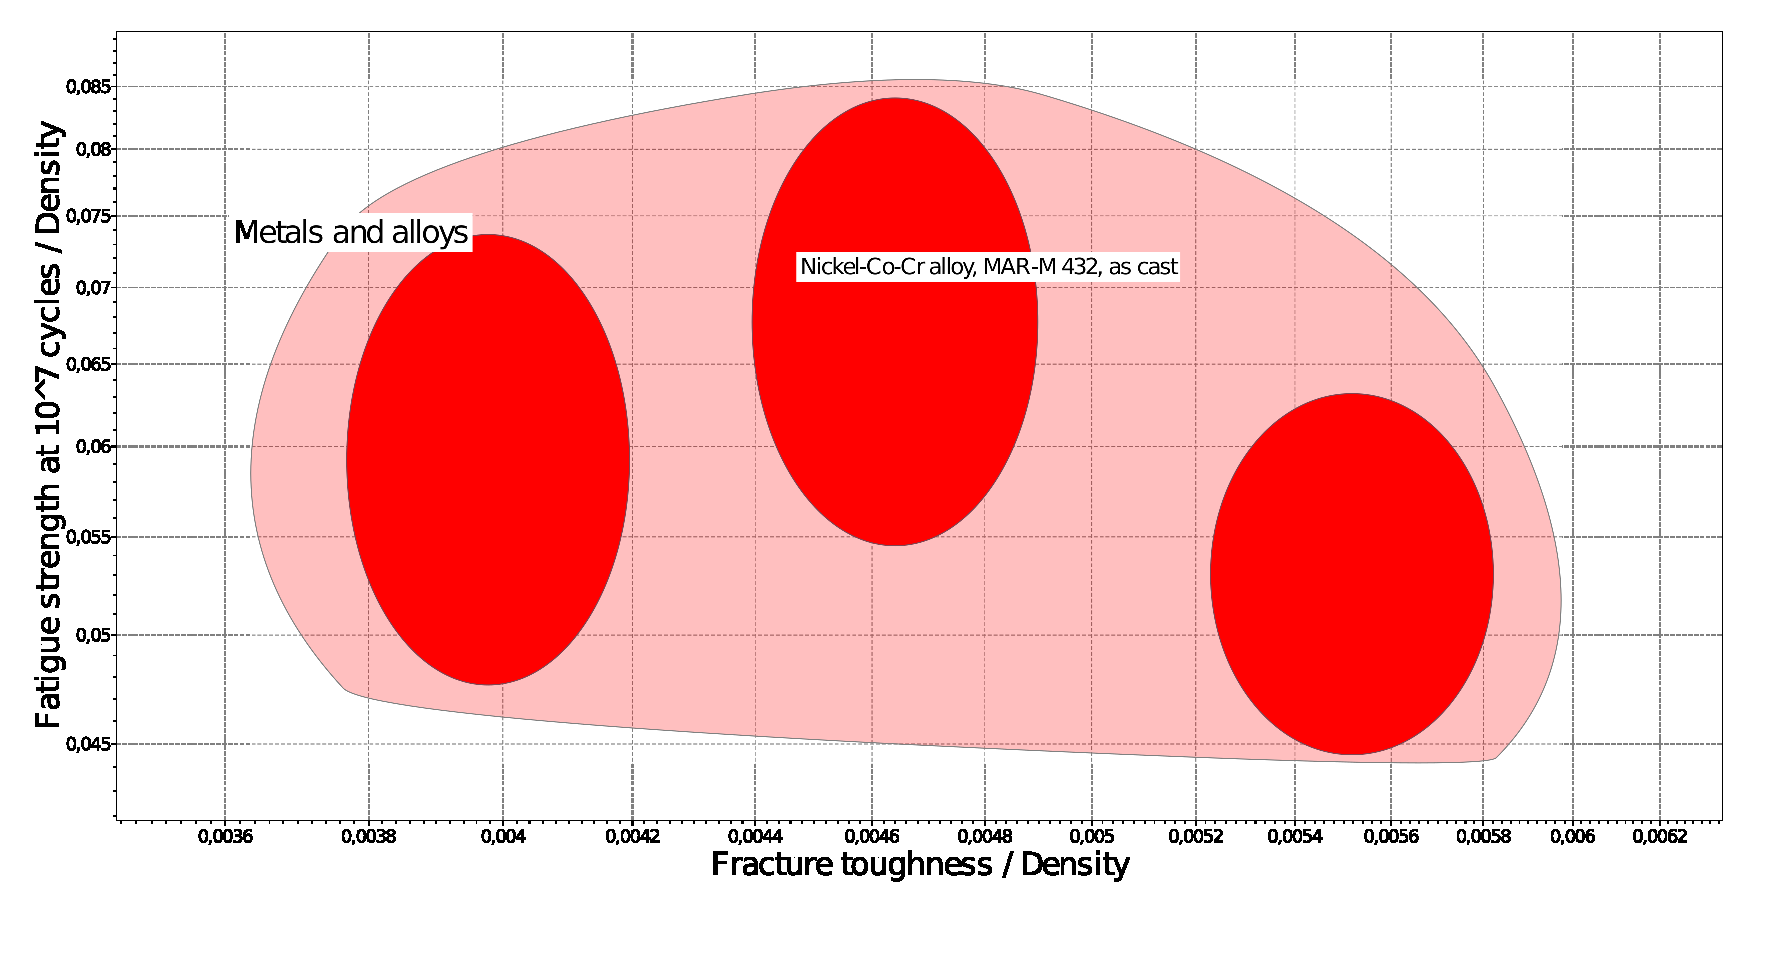
\includegraphics[width=\textwidth]{indici.eps}
            \caption{Fatigue Index vs Fracture Toughness Index}
        \end{figure}

        Come ultimo step, il plot di un indice in funzione dell'altro mette in risalto che \textit{MARM-432}
        occupa mediamente il punto massimo, per cui é stato scelto come materiale finale di progetto, 
        anche in virtú del fatto che si é deciso di dare prioritá alla resistenza a fatica piuttosto che 
        alla fracture toughness, seppur con la consapevolezza che le due grandezze siano correlate.

        É inoltre opportuno far presente che le densitá tra i tre materiali candidati sono assolutamente comparabili, 
        in quanto tutti e tre appartenenti alla categoria delle leghe di Nickel, per cui in realtá si ha 
        quasi un confronto diretto tra \textit{fatigue strength} e \textit{fracture toughness}, dato che in questo specifico 
        scenario la densitá in sé non gioca un ruolo rilevante.

        

    
        \begin{table}[h!]
            \centering
            \begin{tabular}{@{}cc@{}}
            \toprule
            \multicolumn{2}{c}{\textbf{Nickel-Co-Cr alloy, MAR-M 432, as cast}} \\ \midrule
            Al (aluminum)                       & 2.8 \%                         \\
            B (boron)                           & 0.015 \%                       \\
            Co (cobalt)                         & 20 \%                          \\
            Cr (chromium)                       & 15.5 \%                        \\
            Nb (niobium)                        & 2 \%                           \\
            \textit{\textbf{Ni (nickel)}}       & \textit{\textbf{50.3 \%}}      \\
            Ta (tantalum)                       & 2 \%                           \\
            Ti (titanium)                       & 4.3 \%                         \\
            W (tungsten)                        & 3 \%                           \\ \bottomrule
            \end{tabular}
            \caption{Composizione di MAR-M 432}
            \label{tab:marm_composition}
            \end{table}


        \begin{table}[h!]
            \centering
            \resizebox{\textwidth}{!}{
            \begin{tabular}{@{}cc@{}}
            \toprule
            \multicolumn{2}{c}{\textbf{Properties}}                                             \\ \midrule
            Density                                   & $8.05e3 \  -  \ 8.25e3       \ \ \ \ \ \ [\frac{kg}{m^3}         ]  $ \\
            Young's modulus                           & $195    \ -   \  210         \ \ \ \ \ \ [ GPa                   ]  $ \\
            Yield strength (elastic limit)            & $960    \ -   \  1,18e3      \ \ \ \ \ \ [ MPa                   ]  $ \\
            Tensile strength                          & $1,12e3 \    -\     1,37e3   \ \ \ \ \ \ [ MPa                   ]  $ \\
            Fatigue strength at $10^7$ cycles         & $445    \ -   \  685         \ \ \ \ \ \ [ MPa                   ]  $ \\
            Fracture toughness                        & $35,9   \  -  \   39,8       \ \ \ \ \ \ [ MPa \ m^{0.5}         ]  $ \\
            Melting point                             & $1,2e3  \   - \    1,38e3    \ \ \ \ \ \ [ °C                    ]  $ \\
            Maximum service temperature               & $797    \ -   \  1,1e3       \ \ \ \ \ \ [ °C                    ]  $ \\
            Thermal expansion coefficient             & $11     \-    \ 14           \ \ \ \ \ \ [ \frac{\mu strain}{°C} ]  $ \\
            Recycle fraction in current supply (2018) & $28,9   \  -  \   31,9       \ \ \ \ \ \ [ \%                    ]  $ \\ \bottomrule
            \end{tabular}
            }
            \caption{Proprietá di rilievo di MAR-M 432}
            \label{tab:marm_properties}
            \end{table}

        \clearpage

    \subsection{Sviluppi futuri}

    Sicuramente, nei prossimi anni, la manifattura additiva, grazie a tecnologie come l'\textit{EBM}, 
    potrá affermarsi anche in situazioni in cui é richiesto un elevatissimo rateo produttivo. 

    Come giá abbondantemente detto in sezione \ref{Casting}, presenta enormi vantaggi rispetto ad altri 
    metodi tradizionali ed é insostituibile per determinate geometrie troppo complesse. \\
    
    Infatti, attualmente, la maggior parte delle aziende aerospaziali investono molto su questa tecnologia, 
    in molti casi utilizzandola giá per produzioni quantitativamente notevoli, come 
    nel caso di \textit{General Electric}, che affida all'azienda italiana \textit{Avio} la manifattura
    in EBM di palette di turbina per il motore turbofan \textit{GE-90X} \autocite{GE90X_EBM}. \\

    A tale tecnologia si prestano numerose leghe e la ricerca in merito a nuovi materiali ad alte prestazioni (non
    solo metallici)
    che possano sfruttarla al meglio é molto fiorente, come nel caso della superlega Co-Ni10, 
    con cui sono stati ottenuti ottimi risultati, sperimentati anche su provini
    dalla geometria di palette, sia in 
    \textit{selective laser melting} che in \textit{electron beam melting}, per le quali
    le tradizionali superleghe di Nickel tendono a manifestare cricche durante la
    manifattura, dovute alla rapida precipitazione della fase $\gamma^{'}$ \autocite{Co_Ni_EBM}. \\ 

    Si prevede, in conclusione, che la manifattura additiva diventerá lo standard nella produzione di palette
    di turbina, cosí come di una miriade di 
    altre componenti del settore aerospaziale (e non solo) e che i database di materiali come \textit{Granta} verranno conseguentemente aggiornati per 
    meglio includerla ed integrarla nel proprio workflow. 

    

    \clearpage

    \printbibliography
    
\end{document}
